\documentclass{AeroStructure-ERJohnson}
\input crosslink.tex

%\usepackage{showframe}
\def\ShowFrameLinethickness{0.125pt}

\def\harp#1{\smash{\mathord{\buildrel{\lower3pt\hbox{$\scriptscriptstyle\rightharpoonup$}}\over{#1}}}}

\myexternaldocument{App_4P}
\myexternaldocument{Ch01_4P}
\myexternaldocument{Ch02_4P}
\myexternaldocument{Ch03_4P}
\myexternaldocument{Ch04_4P}
\myexternaldocument{Ch05_4P}
%\myexternaldocument{Ch06_4P}
\myexternaldocument{Ch07_4P}
\myexternaldocument{Ch08_4P}
\myexternaldocument{Ch09_4P}
\myexternaldocument{Ch10_4P}
\myexternaldocument{Ch11_4P}
\myexternaldocument{Ch12_4P}
\myexternaldocument{Ch13_4P}
\myexternaldocument{Ch14_4P}
\myexternaldocument{Ch15_4P}
\myexternaldocument{Ch16_4P}
\myexternaldocument{Ch17_4P}
\myexternaldocument{Ch18_4P}


\begin{document}

\mainmatter

\setcounter{page}{143}
\setcounter{chapter}{5}

\chapter{Applications of\break Castigliano's Theorems}\label{ch6}

\section{Coplanar trusses}\label{sec6.1}
\subsection{Castigliano’s first theorem}\label{sec6.1.1}

Consider a truss idealized as an assemblage of uniform bars connected by smooth ball-and-socket joints in three-dimensional trusses, or by smooth hinge joints in a coplanar truss. External forces are assumed to act only at the joints. The line connecting the joints at the end of each bar is assumed to coincide with the reference axis of the bar. Hence, the axial force and strain in each bar is uniform along its length, and the bar is either in tension or compression.


\processfigure{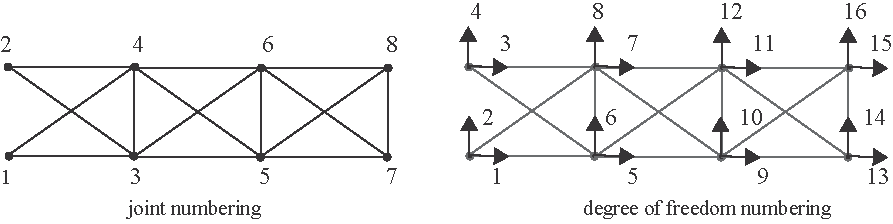
\includegraphics{Figure_6-1.pdf}
}
{\caption{A fifteen-bar truss.}\label{fig6.1}}

A coplanar truss consisting of fifteen bars and eight joints is shown in figure~\ref{fig6.1}. Each joint in a coplanar truss has two degrees of freedom, one horizontal displacement and the one vertical displacement. Hence, there are sixteen displacement degrees of freedom for this truss. At joint $i$, $i=1, 2,\ldots,8$, the horizontal displacement is denoted by $q_{2 i-1}$ and the vertical displacement is denoted by $q_{2 i}$. The positive directions for the displacements and corresponding forces in the fifteen bar truss are shown in figure~\ref{fig6.1}. The original coordinates of the joints and the sixteen displacements completely define the configuration of the truss in the deformed state.

A typical bar in a truss connecting joints labeled $i$ and $j$ is shown in figure~\ref{fig6.2}(a). The location of the bar in a \textit{X-Y} coordinate system is established by the coordinates of joint $i$ ($X_{i}$, $Y_{i}$) and those of joint $j$ ($X_{j}$, $Y_{j}$). The angle of the bar with respect to the $X$-axis is denoted by $\theta$. Trigonometric functions of the angle $\theta$ are related to the coordinates of the joints and length $L$ of the bar by
\begin{align}\label{eq6.1}
\cos \theta=\left(X_{j}-X_{i}\right) / L \quad \sin \theta=\left(Y_{j}-Y_{i}\right) / L \quad L=\sqrt{\left(X_{j}-X_{i}\right)^{2}+\left(Y_{j}-Y_{i}\right)^{2}}.
\end{align}
As shown In figure~\ref{fig6.2}(a), the axial displacement of the bar at joint $i$ is $\bar{q}_{i}$ and that of joint $j$ is $\bar{q}_{j}$. Assume the\break axial displacement $w(z)=\bar{q}_{i}(1-z / L)+\bar{q}_{j}(z / L)$, $0 \leq z \leq L$. The axial strain $\varepsilon_{z z}=w^{\prime}=\left(\bar{q}_{j}-\bar{q}_{i}\right) / L$, and denote\break the elongation $\Delta_{i-j}=\bar{q}_{j}-\bar{q}_{i}$. Also, assume the temperature change is uniform in $z$. From eq.~(\ref{eq3.79}) on page \pageref{eq3.79} the axial force in the bar is
\begin{align}\label{eq6.2}
N_{i-j}=\left(\frac{E A}{L}\right)_{i-j} \Delta_{i-j}-\left(N_{T}\right)_{i-j}.
\end{align}

\processfigure[!t]{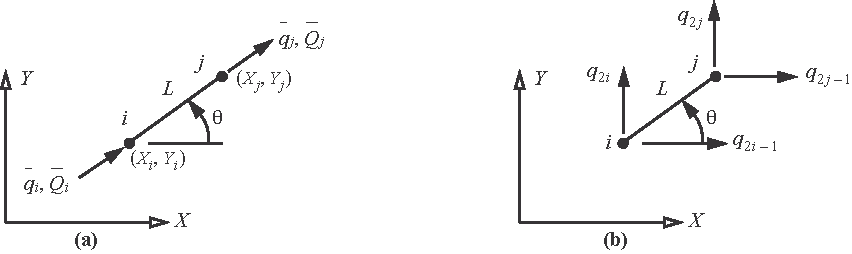
\includegraphics{Figure_6-2.pdf}}{\caption{(a) Truss bar \textit{i-j} subject to axial displacements. (b) Truss bar \textit{i-j} subject to horizontal and vertical displacements.}\label{fig6.2}}

\vspace*{-1pc}

\noindent The differential equation of equilibrium $\frac{dN}{dz}=0$ (eq.~(\ref{eq3.53}) on page \pageref{eq3.53}) is satisfied under assumptions of uniform axial strain and uniform axial change in temperature.The strain energy (\ref{eq5.81}) on page \pageref{eq5.81} of the bar reduces to
\begin{align}\label{eq6.3}
U=\frac{1}{2} \frac{E A}{L} \Delta_{i-j}^{2}-N_{T} \Delta_{i-j}.
\end{align}
Castigliano's first theorem determines the force $\bar{Q}_{i}$ corresponding to displacement $\bar{q}_{i}$, and force $\bar{Q}_{j}$ corresponding to displacement $\bar{q}_{j}$. The results are
\begin{align}\label{eq6.4}
\bar{Q}_{i}=\frac{\partial U}{\partial \bar{q}_{i}}=\frac{E A}{L}\left(\bar{q}_{i}-\bar{q}_{j}\right)+N_{T}\quad \text{and}\quad \bar{Q}_{j}=\frac{E A}{L}\left(-\bar{q}_{i}+\bar{q}_{j}\right)-N_{T}.
\end{align}
Note that $\bar{Q}_{i}+\bar{Q}_{j}=0$, which is the condition of equilibrium.


\processfigure{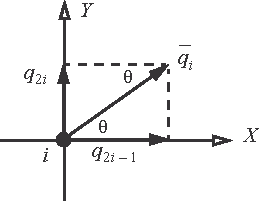
\includegraphics{Figure_6-3.pdf}
}
{\caption{Relation between the displacements components at joint $i$.}\label{fig6.3}}

In figure~\ref{fig6.2}(b) truss displacements of joint $i$ are $\left(q_{2 i-1}, q_{2 i}\right)$ and for joint $j$ are $\left(q_{2 j-1}, q_{2 j}\right)$. At joint $i$ the truss and axial displacements are related by $q_{2 i-1}=\bar{q}_{i} \cos \theta$ and $q_{2 i}=\bar{q}_{i} \sin \theta$ as shown in figure~\ref{fig6.3}. Likewise at joint $j$ $q_{2 j-1}=\bar{q}_{j} \cos \theta$ and $q_{2 j}=\bar{q}_{j} \sin \theta$. These relations can be solved for the axial displacement in terms of the truss displacements to get
\begin{align}\label{eq6.5}
\bar{q}_{i}=q_{2 i-1} \cos \theta+q_{2 i} \sin \theta \quad \bar{q}_{j}=q_{2 j-1} \cos \theta+q_{2 j} \sin \theta.
\end{align}

\pagebreak

\noindent The elongation of the truss bar \textit{i-j} in terms of the joint displacements is
\begin{align}\label{eq6.6}
\Delta_{i-j}=\bar{q}_{j}-\bar{q}_{i}=\left(q_{2 j-1}-q_{2 i-1}\right) \cos \theta+\left(q_{2 j}-q_{2 i}\right) \sin \theta.
\end{align}
The elongation (\ref{eq6.6}) is the sum of the projections of the relative displacements onto the reference axis of the undeformed bar which is depicted in figure~\ref{fig6.4}.

\processfigure{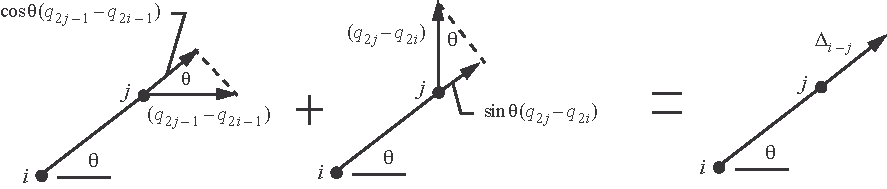
\includegraphics{Figure_6-4.pdf}
}
{\caption{Elongation of the bar as the sum of projections of the relative horizontal and vertical displacements along the direction of the undeformed bar.}\label{fig6.4}}

For the \textit{m-th} bar of the truss shown in figure~\ref{fig6.1}, where, $m = 1, 2,\ldots, 15$, denote its extension stiffness by $(E A / L)_{m}$, its elongation by $\Delta_{m}$, and denote the thermal force by $N_{T m}$. The temperature change is uniform in each bar, but can be different from bar to bar. The relation between bar index $m$ and the joints $i$ and $j$ of the bar are defined by assignment. For example in figure~\ref{fig6.1}, the bar identified by $m = 2$ may be selected as the bar connecting joint 1 to joint 4, so its elongation (\ref{eq6.6}) is
\[
\Delta_{2}=\Delta_{1-4}=\left(q_{7}-q_{1}\right) \cos \theta_{2}+\left(q_{8}-q_{2}\right) \sin \theta_{2}.
\]
The sine and cosine of angle $\theta_2$ are determined from eq.~(\ref{eq6.1}). The strain energy of the assemblage is simply the sum of the strain energies in each bar, where (\ref{eq6.3}) is the energy for one bar. Hence, the total strain energy is
\begin{align}\label{eq6.7}
U=\sum_{m\,=\,1}^{15}\left\{\frac{1}{2}\left(\frac{E A}{L}\right)_{m} \Delta_{m}^{2}-N_{T_{m}} \Delta_{m}\right\} .
\end{align}
 The displacements $q_{n}$ and the corresponding forces $Q_{n}$, $n=1,2, \ldots, 16$, used in the formulation of Castigliano's theorem are the displacements and corresponding forces at the joints. Hence, Castigliano's first theorem for the truss shown in figure~\ref{fig6.1} is
\begin{align}\label{eq6.8}
Q_{n}=\sum_{m\,=\,1}^{15}\left[\left(\frac{E A}{L}\right) \Delta_{m}-N_{T m}\right] \frac{\partial \Delta_{m}}{\partial q_{n}} \quad n=1,2, \ldots, 16.
\end{align}

\begin{example*}[Three-bar coplanar truss]\label{ex6.1}The coplanar truss shown in figure~\ref{fig6.5} consists of three bars ($m$ = 1, 2, 3) and four joints 1, 2, 3, 4. Beginning joint $i$ and end joint $j$ for each bar are listed in the figure. Joints 2, 3, and 4 are fixed so their displacements equal zero, and joint 1 is movable. The change in the thermal force in each bar is equal to zero. The spring stiffness of the bars are denoted by $(E A / L)_{m}$. Determine the $2\times 2$ stiffness matrix using Castigliano's first theorem.

\processfigure{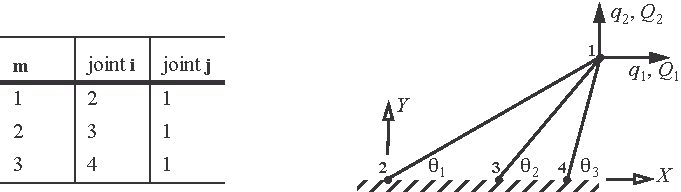
\includegraphics{Figure_6-5.pdf}
}
{\caption{Three-bar truss.}\label{fig6.5}}

\subsubsection{Solution.} The elongation of each bar as determined from eq.~(\ref{eq6.6}) is
\begin{equation*}
\Delta_{m}=\cos \left(\theta_{m}\right) q_{1}+\sin \left(\theta_{m}\right) q_{2} \quad m=1,2,3.
\tag{a}
\end{equation*}
Castigliano's theorem (\ref{eq6.8}) applied to this example yields
\begin{gather*}
Q_{1}=\sum_{m\,=\,1}^3\left(\frac{E A}{L}\right)_{m}\left[\cos \left(\theta_{m}\right) q_{1}+\sin \left(\theta_{m}\right) q_{2}\right]\left[\cos \left(\theta_{m}\right)\right] \tag{b}\\
Q_{2}=\sum_{m\,=\,1}^3\left(\frac{E A}{L}\right)_{m}\left[\cos \left(\theta_{m}\right) q_{1}+\sin \left(\theta_{m}\right) q_{2}\right]\left[\sin \left(\theta_{m}\right)\right]\tag{c}
\end{gather*}
These results are written in the matrix form
\begin{equation*}
\left[\begin{array}{@{}l@{}}Q_{1} \\Q_{2}\end{array}\right]=\left[\begin{array}{@{}ll@{}}k_{11} & k_{12} \\k_{21} & k_{22}\end{array}\right]\left[\begin{array}{@{}l@{}}q_{1} \\q_{2}\end{array}\right],\tag{d}
\end{equation*}
where the elements of the stiffness matrix are
\begin{equation*}
k_{11}=\sum_{m\,=\,1}^{3}\left(\frac{E A}{L}\right)_{m}\cos^{2}\left(\theta_{m}\right) \quad k_{22}=\sum_{m\,=\,1}^{3}\left(\frac{E A}{L}\right)_{m} \sin^{2}\left(\theta_{m}\right) \quad k_{12}=k_{21}=\sum_{m\,=\,1}^{3}\left(\frac{E A}{L}\right)_{m} \cos \left(\theta_{m}\right) \sin \left(\theta_{m}\right).\tag{e}
\end{equation*}
Note that this example is statically indeterminate, since there are only two equilibrium equations at the movable joint 1 but three unknown bar forces. For specified nodal forces $Q_1$ and $Q_2$, matrix eq. (\textbf{d}) is solved for the nodal displacements $q_1$ and $q_2$. From eq.~(\textbf{a}) the elongation of each bar is then computed, and from these elongations the bar forces are determined from
\begin{align*}
N_{m}=\left(\frac{E A}{L}\right)_{m} \Delta_{m} \quad m=1,2,3.\tag{f}
\end{align*}\hfill\qed
\end{example*}

\clearpage

\begin{example*}[Three-bar truss with lack of fit]\label{ex6.2}Consider the same three bar-truss of example 6.1, but now assume that bar 1 was too short and had to be stretched an amount $\bar{\Delta}_{1}$ in order to connect it to joint 1. This is a case of lack of fit, and lack of fit is common in the fabrication of structures. That is, before the external loads are applied ($Q_{1}=Q_{2}=0$), the truss bars experience initial forces due to the lack of fit of bar 1. Determine the initial forces in the bars using Castigliano's first theorem.

\subsubsection{Solution.} Lack of fit can be included in the energy analysis by modifying the specified thermal force term in the strain energy (\ref{eq6.7}). For uniform material properties and uniform change in temperature, the thermal force in a truss bar is $N_{T}=E A \alpha \Delta T$. (Refer to eq.~(\ref{eq3.75}) on page \pageref{eq3.75}.) The factor $\alpha \Delta T=\varepsilon_{0}$ is the initial strain due to the temperature change. Note $\varepsilon_{0}$ is dimensionless. Now interpret $\varepsilon_{0}$ as the initial strain specified due to lack of fit. The initial strain due to the specified displacement $\bar{\Delta}$ required to connect a bar to a joint is $\varepsilon_{0}=\bar{\Delta}/ L$. Let
$N_{T} \rightarrow N_{\bar{\Delta}}=E A(\bar{\Delta}/ L)$. The strain energy is modified to
\begin{equation*}
U=\sum_{m\,=\,1}^3\left\{\frac{1}{2}\left(\frac{E A}{L}\right)_{m} \Delta_{m}^{2}-N_{\bar{\Delta} m}\Delta_{m}\right\}.\tag{a}
\end{equation*}
The specified initial strain is only for bar 1, so
\begin{equation*}
U=\sum_{m\,=\,1}^3 \frac{1}{2}\left(\frac{E A}{L}\right)_{m} \Delta_{m}^{2}-\left(\frac{E A}{L}\right)_{1} \bar{\Delta}_{1} \Delta_{1}.\tag{b}
\end{equation*}
Castigliano's theorem (\ref{eq6.8}) leads to
\begin{gather}
Q_{n}=\sum_{m\,=\,1}^3\left[\left(\frac{E A}{L}\right) \Delta_{m}\right] \frac{\partial \Delta_{m}}{\partial q_{n}}-\left(\frac{E A}{L}\right)_{1} \bar{\Delta}_{1}\left(\frac{\partial \Delta_{1}}{\partial q_{n}}\right) \quad n=1,2.\tag{c}
\end{gather}
The matrix form of eq. (\textbf{c}) is
\begin{gather}
\left[\begin{array}{@{}l@{}}Q_{1} \\Q_{2}\end{array}\right]=\left[\begin{array}{@{}ll@{}}k_{11} & k_{12} \\k_{21} & k_{22}\end{array}\right]\left[\begin{array}{@{}l@{}}q_{1} \\q_{2}\end{array}\right]-\left(\frac{E A}{L}\right)_{1}\bar{\Delta}_{1}\left[\begin{array}{@{}l@{}}\cos \left(\theta_{1}\right) \\\sin \left(\theta_{1}\right)\end{array}\right].\tag{d}
\end{gather}
Elements of the stiffness matrix are the same as given by eq. (\textbf{e}) of example 6.1. Set $Q_{1}=0$ and $Q_{2}=0$, since no external forces are applied to the joint just after assembly. Then solve the matrix equation (\textbf{d}) for the joint displacements to get
\begin{equation*}
\left[\begin{array}{@{}l@{}}q_{1} \\q_{2}\end{array}\right]=\left[\begin{array}{@{}ll@{}}k_{11} & k_{12} \\k_{21} & k_{22}\end{array}\right]^{-1}\left[\begin{array}{@{}c@{}}\cos \left(\theta_{1}\right) \\\sin \left(\theta_{1}\right)\end{array}\right]\left(\frac{E A}{L}\right)_{1} \bar{\Delta}_{1}.\tag{e}
\end{equation*}
From this solution for the displacements we can calculate the elongation of each bar after assembly from eq. (\textbf{a}) in example~6.1. The initial bar forces after assembly are computed from
\begin{equation*}
N_{1}=\left(\frac{E A}{L}\right)_{1}\left(\Delta_{1}-\bar{\Delta}_{1}\right) \quad N_{2}=\left(\frac{E A}{L}\right)_{2} \Delta_{2} \quad N_{3}=\left(\frac{E A}{L}\right)_{3} \Delta_{3}.\tag{f}
\end{equation*}

\vspace*{-1pc}

A specific case: $\theta_{1}=30^{\circ}$, $\theta_{2}=45^{\circ}$, $\theta_{3}=60^{\circ}$, and $E A$ is the same for each bar. Take $L_{1}=L$, so that $L_{2}=L / \sqrt{2}$, and $L_{3}=L /(\sqrt{3})$. The solution for the displacements from eq. (\textbf{b}) are $q_{1}=1.458 \bar{\Delta}_{1}$ and $q_{2}=-\bar{\Delta}_{1}$. The elongations are $\Delta_{1}=0.763 \bar{\Delta}_{1}$, $\Delta_{2}=0.324 \bar{\Delta}_{1}$, and $\Delta_{3}=-0.137 \bar{\Delta}_{1}$, and the bar forces from eq. (\textbf{f}) are
\begin{equation}
N_{1}=-0.237 E A\left(\bar{\Delta}_{1} / L\right) \quad N_{2}=0.458 E A\left(\bar{\Delta}_{1} / L\right) \quad N_{3}=-0.237 E A\left(\bar{\Delta}_{1} / L\right).\tag{g}
\end{equation}\hfill\qed
\end{example*}

\subsection{Castigliano's second theorem for a statically determinate truss}\label{sec6.1.2}

\begin{example*}[Truss displacements]\label{ex6.3}The truss shown in figure~\ref{fig6.6} consists of three bars labeled 1-2, 1-3, and 2-3. Joint 1 is a fixed pin, and pin joint 3 is free to move vertically but not horizontally. A downward applied force of a 84,000 N acts at joint 2. The cross-sectional areas of bars are $A_{1-2}=900\,\mathrm{mm}^{2}$, $A_{1-3}=300\,\mathrm{mm}^{2}$, and $A_{2-3}=1,200\,\mathrm{mm}^{2}$. Each bar has a modulus of elasticity \textit{E} = 70,000 N/mm$^2$. The degree of freedom numbering is shown the figure. Determine displacements $q_3$ and $q_4$ by Castigliano's second theorem

\begin{figure}[!h]
\centerline{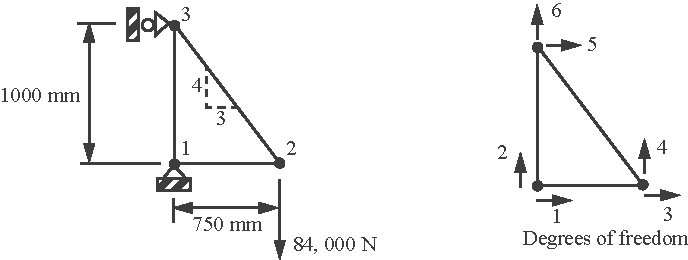
\includegraphics{Figure_6-6.pdf}}
\caption{A statically determinate three-bar truss.}\label{fig6.6}
\end{figure}

\subsubsection{A note on static determinacy:} Let $m\,{=}\,$the number of unknown bar forces, $r\,{=}\,$the number of support reactions, and let $j\,{=}\,$the number of joints. There are two independent equilibrium equations per joint. For a statically determinate truss, the number of unknown forces is equal to number of independent equilibrium equations (i.e., $2j = m + r$). For the truss in this example $j = 3$, $m = 3$, and $r = 3$. So it is statically determinate. For the truss in example 6.1, $j = 3$, $m = 3$, and $r = 6$, and $6 < 3 + 6$. So the truss in example 6.1 is statically indeterminate.

\subsubsection{Solution.} Free body diagrams of joints 2 and 3 are shown figure~\ref{fig6.7}. The diagrams are drawn assuming each bar is in tension, so the reaction of the bar force acting on a joint is an arrow aligned with the bar and pointing away from the joint. The objective is to determine each bar force in terms of external forces $Q_3$ and $Q_4$. Note that $Q_3 = 0$ and $Q_4 = -84{,}000$~N, but we will wait to substitute these numerical values after the derivatives are evaluated in Castigliano's second theorem.

\begin{figure}[!h]
\centerline{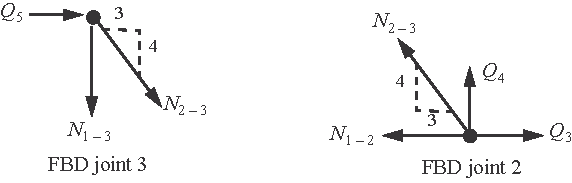
\includegraphics{Figure_6-7.pdf}}
\caption{Free body diagrams of two joints of the 3-bar truss.}\label{fig6.7}
\end{figure}

The only contribution to the complementary strain energy in (\ref{eq5.84}) on page \pageref{eq5.84} is the axial normal force $N$, which is spatially uniform along the length of the bar. Also, there is no change in temperature from the\vadjust{\vspace*{6pt}\pagebreak} reference state. Hence, the complementary strain energy for the truss is
\begin{equation*}
U^{*}=\frac{1}{2}\left[\left(\frac{L}{E A}\right)_{1-2} N_{1-2}^{2}+\left(\frac{L}{E A}\right)_{1-3} N_{1-3}^{2}+\left(\frac{L}{E A}\right)_{2-3} N^{2}_{2-3}\right],\tag{a}
\end{equation*}
Castigliano's second theorem for the displacement $q_3$ is
\begin{equation*}
q_{3}=\frac{\partial U^{*}}{\partial Q_{3}}=\left(\frac{L}{E A}\right)_{1-2} N_{1-2} \frac{\partial N_{1-2}}{\partial Q_{3}}+\left(\frac{L}{E A}\right)_{1-3} N_{1-3} \frac{\partial N_{1-3}}{\partial Q_{3}}+\left(\frac{L}{E A}\right)_{2-3} N_{2-3} \frac{\partial N_{2-3}}{\partial Q_{3}}.\tag{b}
\end{equation*}

\vspace*{-1pc}

\noindent The terms in eq. \textbf{(b)} are listed in table~\ref{tab6.1}. Replace the derivatives of the bar forces with their values listed in the table to get

\begin{table}[!h]%T1
\processtable{Terms in Castigliano's theorem for displacements $\textit{q}_{\bf 3}$ and $\textit{q}_{\bf 4}$\label{tab6.1}}{%
\begin{tabular}{@{}lllllll@{}}
\toprule
\colhead{Bar} &\colhead{L, mm} &\colhead{A, mm$^{\bf 2}$} &\colhead{L/(EA), mm/N} &\colhead{N} & \colhead{$\partial N / \partial Q_{3}$} & \colhead{$\partial N / \partial Q_{4}$} \\
\midrule
1-2 &750 &900 &$11.90 \times 10^{-6}$ &$Q_{3}+3 Q_{4}/4$ &1 &3/4 \\
1-3 &1000 &300 &$47.62 \times 10^{-6}$ &$Q_{4}$ &0 &1 \\
2-3 &1250 &1200 &$14.88 \times 10^{-6}$ &$-5 Q_{4}/4$ &0 &$-5/4$ \\
\botrule
\end{tabular}}{}
\vspace*{-1pc}
\end{table}

\vspace*{-1pc}

\begin{equation*}
q_{3}=\left(\frac{L}{E A}\right)_{1-2} N_{1-2}(1)+\left(\frac{L}{E A}\right)_{1-3} N_{1-3}(0)+\left(\frac{L}{E A}\right)_{2-3} N_{2-3}(0).\tag{c}
\end{equation*}
Substitute the equation for bar force $N_{1-2}$ from the table in the previous equation and note that $Q_{3}=0$ and $Q_{4}=-84{,}000$~N to get
\begin{equation*}
q_{3}=\left(\frac{L}{E A}\right)_{1-2}\left(Q_{3}+3 Q_{4}/4\right)=\left(11.90\times 10^{-6}\,\mathrm{mm}/ \mathrm{N}\right)\left(0+\frac{3}{4}(-84{,}000\,\mathrm{N})\right)=-0.750\,\mathrm{mm}.\tag{d}
\end{equation*}
Castigliano's second theorem for the displacement $q_4$ is
\begin{equation*}
q_{4}=\frac{\partial U^{*}}{\partial Q_{4}}=\left(\frac{L}{E A}\right)_{1-2} N_{1-2} \frac{\partial N_{1-2}}{\partial Q_{4}}+\left(\frac{L}{E A}\right)_{1-3} N_{1-3} \frac{\partial N_{1-3}}{\partial Q_{4}}+\left(\frac{L}{E A}\right)_{2-3} N_{2-3} \frac{\partial N_{2-3}}{\partial Q_{4}}.\tag{e}
\end{equation*}
Replace the bar forces and their derivatives in eq. (\textbf{e}) with their values listed in table~\ref{tab6.1} to get
\begin{equation*}
q_{4}=\left(\frac{L}{E A}\right)_{1-2}\left(0+3 Q_{4}/4\right)\left(\frac{3}{4}\right)+\left(\frac{L}{E A}\right)_{1-3}\left(Q_{4}\right)(1)+\left(\frac{L}{E A}\right)_{2-3}\left(-5 Q_{4}/4\right)\left(-\frac{5}{4}\right).\tag{f}
\end{equation*}
Substitute numerical values into eq. (\textbf{f}) to get
\begin{equation*}
q_{4}=\left[(11.90 \times 10^{-6}\,\mathrm{mm} / \mathrm{N}) \frac{9}{16}+(47.62 \times 10^{-6}\,\mathrm{mm} / \mathrm{N})+(14.88 \times 10^{-6}\,\mathrm{mm} / \mathrm{N}) \frac{25}{16}\right](-84{,}000\,\mathrm{N}).\tag{g}
\end{equation*}
The final result from eq. (\textbf{g}) is
\begin{align*}
q_{3}=-0.750\,\mathrm{mm} \quad q_{4}=-6.516\,\mathrm{mm}  \tag{h}
\end{align*}\hfill\qed
\end{example*}

\section{Beam structures}\label{sec6.2}

\begin{example*}[Cross-sectional properties of a thin-walled tube]\label{ex6.4}The cross section is a thin-walled tube with a circular contour of radius $a$ and wall thickness $t$. as shown in figure~\ref{fig6.8}.

\begin{wrapfigure}[10]{L}{92.07pt}
\vspace{-19pt}
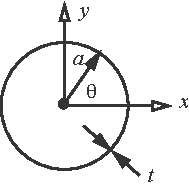
\includegraphics{Figure_6-8.pdf}
\caption{ \label{fig6.8}}
\end{wrapfigure}


\subsubsection{Solution.} The $x$- and $y$- axes are axes of symmetry in the cross section, so the centroid and shear center coincide with the center of the circular contour. The parametric coordinates of the circular contour are $x=a \cos \theta$ and $y=a \sin \theta$, and the arc length along the contour $s=a \theta$; $0 \leq \theta \leq 2 \pi$. The cross-sectional area and first area moments are
\begin{equation*}
A=\int_{0}^{2 \pi} t a d \theta=2 \pi a t \quad Q_{x}=\int_{0}^{2 \pi} y {tad} \theta=0 \quad Q_{y}=\int_{0}^{2 \pi} x t a d \theta=0.\tag{a}
\end{equation*}
The first area moments equal zero since the center of thee circle is the centroid. The second area moments are
\begin{equation*}
I_{x x}=\int_{0}^{2 \pi} y^{2} t a d \theta=\pi a^{3} t \quad I_{y y}=\int_{0}^{2 \pi} x^{2} t a d \theta=\pi a^{3} t \quad I_{x y}=\int_{0}^{2 \pi} x y t a d \theta=0.\tag{b}
\end{equation*}
Since the product area moment is zero, then coefficients $n_{x}=n_{y}=0$ and $k=1$ from eq.~(\ref{eq4.4}) on page \pageref{eq4.4}. To compute the transverse shear compliances given in eq.~(\ref{eq4.30}) on page \pageref{eq4.30}, we need to compute the distribution functions from eq.~(\ref{eq4.19}) and eq.~(\ref{eq4.26}). The distribution functions for the first area moments for a segment of the contour from $s=0$ to $s=a \theta$ are given by
\begin{equation*}
Q_{x}(\theta)=\int_{0}^{\theta} y {tad} \theta=a^{2} t(1-\cos \theta) \quad Q_{y}(\theta)=\int_{0}^{\theta} x t a d \theta=a^{2} t \sin \theta.\tag{c}
\end{equation*}
The coordinates normal and tangent to the contour with respect to the shear center are
\begin{equation*}
r_{n}=x\left(\frac{1}{a} \frac{d y}{d \theta}\right)-y\left(\frac{1}{a} \frac{d x}{d \theta}\right)=a \quad r_{t}=x\left(\frac{1}{a} \frac{d x}{d \theta}\right)+y \frac{1}{a} \frac{d y}{d \theta}=0.\tag{d}
\end{equation*}
(Refer to eq.~(\ref{eq3.10}) on page \pageref{eq3.10}.) The area enclosed by the contour is
\begin{equation*}
A_{c}=\frac{1}{2} \int_{0}^{2 \pi} r_{n} a d \theta=\pi a^{2}.\tag{e}
\end{equation*}
The shear flow distribution functions given by eqs.~(\ref{eq4.19}) and (\ref{eq4.26}) on page \pageref{eq4.19} for the closed section are
\begin{gather*}
F_{x}=\frac{1}{I_{y y}}\left[Q_{y}(\theta)-\frac{1}{2 A_{c}} \int_{0}^{2 \pi} r_{n} Q_{y}(\theta) a d \theta\right]=\frac{a^{2} t \sin \theta}{I_{y y}}=\frac{\sin \theta}{a \pi}, \ \text{and}\tag{f}\\
F_{y}=\frac{1}{I_{x x}}\left[Q_{x}(\theta)-\frac{1}{2 A_{c}} \int_{0}^{2 \pi} r_{n} Q_{x}(\theta) a d \theta\right]=-\left(\frac{a^{2} t}{I_{x x}}\right) \cos \theta=\frac{-\cos \theta}{a \pi}.\tag{g}
\end{gather*}
Finally, the transverse shear compliances are
\begin{gather*}
c_{x x}=\frac{1}{G} \int_{0}^{2 \pi} F_{x}^{2}(\theta) a d \theta=\frac{\pi a^{5} t}{G I_{y y}^{2}}=\frac{1}{\pi a t G} \quad c_{y y}=\frac{1}{G t} \int_{0}^{2 \pi} F_{y}^{2}(\theta) a d \theta=\frac{1}{\pi a t G},\ \text{and} \tag{h}\\
c_{x y}=\frac{1}{G t} \int_{0}^{2 \pi}\left[F_{x}(\theta) F_{y}(\theta)\right] a d \theta=0.\tag{i}
\end{gather*}
For a uniform shear modulus around the contour, the torsion constant is determined from eq.~(\ref{eq3.161}) on page~\pageref{eq3.161}~as
\begin{equation*}
J=\frac{4 A_{c}^{2}}{\oint \frac{d s}{t}}=\frac{4\left(\pi a^{2}\right)^{2}}{\frac{2 \pi a}{t}}=2 \pi a^{3} t.\tag{j}
\end{equation*}\hfill\qed
\end{example*}

\vspace*{-1pc}

\subsection{Castigliano's second theorem}\label{sec6.2.1}

\begin{example*}[Thin-walled tube subject to radiant heating]\label{ex6.5}A common structural member in orbiting space structures is a thin-walled tube. Tubes are used as truss members and for satellite booms. Solar heating combined with heat conduction results in the distribution of temperature around the perimeter and along the length of the tube. The data in this example is for an aluminum 6061-T6 tube taken from Thornton (1996, pp. 118--121).

\begin{wrapfigure}[10]{R}{136.14pt}
\vspace{-19pt}
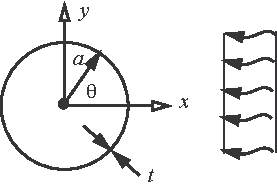
\includegraphics{Figure_6-9.pdf}
\caption{Radiant heating of a tube. \label{fig6.9}}
\end{wrapfigure}

A thin-walled tube with a circular contour of radius $a$, and wall thickness $t$ is subjected to radiant heating as shown in figure~\ref{fig6.9}. The tube is cantilevered, that is, fixed at $z = 0$ and free at $z =L$, where $L$ is the length of tube. The change in temperature from the reference state is uniform along the length but it varies around the perimeter. and is specified by
\begin{equation*}
\Delta T(\theta)=\bar{T}+T_{m} \cos \theta \quad \theta \in[0,2 \pi].\tag{a}
\end{equation*}
where the average temperature is denoted by $\bar{T}$ and the perturbation in temperature is denoted by $T_{m}$. Data for this example are listed in table~\ref{tab6.2}.

\begin{table}[!h]%T2
\processtable{Numerical data for example~6.5\label{tab6.2}}{%
\begin{tabular}{@{}ll|ll@{}}
\toprule\\[-15.5pt]
& & \\[-6pt]
radius &$a=0.03812\,\mathrm{m}$ &Poisson's ratio &$v=0.33$ \\
wall thickness &$t=7.14 \times 10^{-4}\,\mathrm{m}$ &coefficient of thermal expansion &$\alpha=23 \times 10^{-6\,\circ} ~K$ \\
tube length &$L=0.8\,\mathrm{m}$ &average temperature &$\bar{T}=462^{\circ} K$ \\
modulus of elasticity &$E=68.3~\mathrm{GPa}$ &perturbation temperature &$T_{m}=34^{\circ} K$ \\[-3pt]
& & \\[-3.5pt]
\botrule
\end{tabular}}{}
\vspace*{-1pc}
\end{table}

Determine the displacements $q_1$ and $q_3$, and rotation $q_5$ of the cross section at the free end using Castigliano's second theorem. The degree of freedom numbering is shown in figure~\ref{fig6.10}.


\processfigure{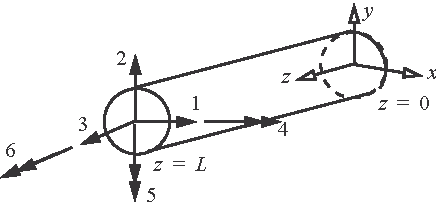
\includegraphics{Figure_6-10.pdf}
}
{\caption{Degree of freedom numbering at the free end of the cantilever tube.}\label{fig6.10}}

\subsubsection{Solution.} From eqs. (\ref{eq5.83}) to (\ref{eq5.85}) on page \pageref{eq5.83} the complementary strain energy in this example is
\begin{equation*}
U^{*}=\frac{1}{2} \int_{0}^{L}\left[\frac{\left(N+N_{T}\right)^{2}}{E A}+\frac{\left(M_{x}+M_{x T}\right)^{2}}{E I_{x x}}+\frac{\left(M_{y}+M_{y T}\right)^{2}}{E I_{y y}}+c_{x x} V_{x}^{2}+c_{y y} V_{y}^{2}+\frac{M_{z}^{2}}{G J}\right] d z.\tag{b}
\end{equation*}
The cross-sectional properties were determined in example~6.4, and they are
\begin{gather*}
A=2 \pi a t=2 \pi(0.03812\,\mathrm{m})(7.14 \times 10^{-4}\,\mathrm{m})=171.014 \times 10^{-6}\,\mathrm{m}^{2},
\tag{c}\\
I_{x x}=I_{y y}=\pi a^{3} t=\pi(0.03812\,\mathrm{m})^{3}(7.14 \times 10^{-4}\,\mathrm{m})=124.25 \times 10^{-9}\,\mathrm{m}^{4},\ \text{and}\ J=2 \pi a^{3} t=248.50 \times 10^{-9}\,\mathrm{m}^{4}.\tag{d}
\end{gather*}
The shear modulus is given by the isotropic formula $G=E /(2(1+v))=25.6~\mathrm{GPa}$, so the transverse shear compliances are
\begin{equation*}
c_{x x}=c_{y y}=\frac{1}{\pi a t G}=\frac{1}{\pi(0.03812\,\mathrm{m})\left(7.14 \times 10^{-4}\,\mathrm{m}\right)\left(25.6 \times 10^{9}\,\mathrm{N} / \mathrm{m}^{2}\right)}=\frac{456.61 \times 10^{-9}}{\mathrm{~N}}.\tag{e}
\end{equation*}
The thermal axial force is given by eq.~(\ref{eq3.75}) on page \pageref{eq3.75}, and thermal moments are given in eq.~(\ref{eq3.78}). Material properties are uniform along the contour and $x=a \cos \theta$, and $y=a \sin \theta$ in the thermal action formulas. The results for these thermal actions are
\begin{align*}
&N_{T}=E \alpha \int_{0}^{2 \pi} \Delta T t a d \theta=2 \pi a t E \alpha \bar{T} \quad M_{x T}=E \alpha \int_{0}^{2 \pi} \Delta T y t a d \theta=0 \quad M_{y T}=E \alpha \int_{0}^{2 \pi} \Delta T x t a d \theta=\pi a^{2} t E \alpha T_{m},&\tag{f} \\
&N_{T}=2 \pi(0.03812\,\mathrm{m})(7.14 \times 10^{-4}\,\mathrm{m})(68.3 \times 10^{9}\,\mathrm{N} / \mathrm{m}^{2})(23 \times 10^{-6}{}^{\circ} ~K)(462^{\circ}~K)=124.11 \times 10^{3}\,\mathrm{N},\ \text{and}& \tag{g} \\
&M_{y T}=\pi(0.03812\,\mathrm{m})^{2}(7.14 \times 10^{-4}\,\mathrm{m})(68.3 \times 10^{9}\,\mathrm{N} / \mathrm{m}^{2})(23 \times 10^{-6}{ }^{\circ} K)(34^{\circ} ~K)=174.10\,\mathrm{N}-\mathrm{m}.&\tag{h}
\end{align*}
The free body diagram of the tube in the \textit{x-z} plane is shown in figure~\ref{fig6.11}. Generalized forces $Q_1$, $Q_3$, and $Q_5$ are introduced at the free end to facilitate computing the corresponding displacements via Castigliano's theorem, and they are set equal to zero at the end of the procedure (i.e., they are fictitious actions).

\processfigure{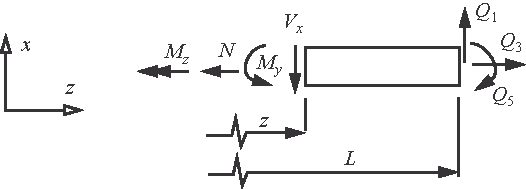
\includegraphics{Figure_6-11.pdf}
}
{\caption{Fictitious actions acting at the free end of the cantilever tube.}\label{fig6.11}}


Equilibrium of the free body diagram in the \textit{x-z} plane yields
\begin{equation*}
N=Q_{3} \quad V_{x}=Q_{1} \quad M_{y}=Q_{5}-Q_{1}(L-z) \quad M_{z}=0 \quad z \in[0, L].\tag{i}
\end{equation*}
Since generalized forces $Q_{2}=Q_{4}=0$, equilibrium in the \textit{y-z} plane yields $V_{y}=M_{x}=0$ for $z \in[0, L]$. The complementary strain energy reduces to
\begin{equation*}
U^{*}=\frac{1}{2} \int_{0}^{L}\left[\frac{\left(Q_{3}+N_{T}\right)^{2}}{E A}+\frac{\left[Q_{5}-Q_{1}(L-z)+M_{y T}\right]^{2}}{E I_{y y}}+\frac{Q_{1}^{2}}{\pi a t G}\right] d z.\tag{j}
\end{equation*}
\vspace*{6pt}
\clearpage

\noindent Displacement $q_1$ is determined\vspace*{-3pt} from
\begin{align*}
q_{1}=\frac{\partial U^{*}}{\partial Q_{1}}=\int_{0}^{L} &\left[\frac{\left(Q_{3}+N_{T}\right)}{E A} \frac{\partial\left(Q_{3}+N_{T}\right)}{\partial Q_{1}}+\frac{\left[Q_{5}-Q_{1}(L-z)+M_{y T}\right]}{E I_{y y}} \frac{\partial\left[Q_{5}-Q_{1}(L-z)+M_{y T}\right]}{\partial Q_{1}} \right.\nonumber \\
&\quad \left. +\frac{Q_{1}}{\pi a t G}\left(\frac{\partial Q_{1}}{\partial Q_{1}}\right)\right] d z,\tag{k}
\end{align*}
where we interchanged the derivative and integral since our functions are continuous. Performing the derivative inside the integral we\vspace*{-3pt} get
\begin{equation*}
q_{1}=\frac{1}{E I_{y y}} \int_{0}^{L}\left[Q_{5}-Q_{1}(L-z)+M_{y T}\right][-(L-z)] d z+\frac{1}{\pi a t G} \int_{0}^{L} Q_{1}(1) d z.\tag{l}
\end{equation*}
Now set $Q_1$ and $Q_5$ equal to zero and\vspace*{-3pt} find
\begin{equation*}
q_{1}=\left(\frac{1}{E I_{y y}}\right) \int_{0}^{L} M_{y T}[-(L-z)] d z=\frac{-L^{2} M_{y T}}{2 E I_{y y}}=\frac{-(0.8\,\mathrm{m})^{2}(174.10\,\mathrm{N}\mbox{-}\mathrm{m})}{2\left(68.3 \times 10^{9}\,\mathrm{N} / \mathrm{m}^{2}\right)\left(124.25 \times 10^{-9}\,\mathrm{m}^{4}\right)}=-6.565 \times 10^{-3}\,\mathrm{m}.\tag{m}
\end{equation*}
Axial displacement $q_3$ is given\vspace*{-3pt} by
\begin{align*}
q_{3}=\frac{\partial U^{*}}{\partial Q_{3}}=\int_{0}^{L}&\left[\frac{\left(Q_{3}+N_{T}\right)}{E A} \frac{\partial\left(Q_{3}+N_{T}\right)}{\partial Q_{3}}+\frac{\left[Q_{5}-Q_{1}(L-z)+M_{y T}\right]}{E I_{y y}} \frac{\partial \left[Q_{5}-Q_{1}(L-z)+M_{y T}\right]}{\partial Q_{3}} \right.\nonumber\\
&\quad\left.+\frac{Q_{1}}{\pi a t G}\left(\frac{\partial Q_{1}}{\partial Q_{3}}\right)\right] d z.\tag{n}
\end{align*}
Since $Q_3 = 0$, the latter equation reduces\vspace*{-3pt} to
\begin{equation*}
q_{3}=\left.\left(\frac{1}{E A}\right) \int_{0}^{L}\left(Q_{3}+N_{T}\right)(1) d z\right|_{Q_{3}=0}=\frac{L}{E A} N_{T}=\frac{(0.8\,\mathrm{m})\left(124.11 \times 10^{3}\,\mathrm{N}\right)}{\left(68.3 \times 10^{9}\,\mathrm{N} / \mathrm{m}^{2}\right)\left(171.014 \times 10^{-6}\,\mathrm{m}^{2}\right)}=8.5 \times 10^{-3}\,\mathrm{m}.\tag{o}
\end{equation*}
Finally, the rotation in radians about the $y$-axis is given\vspace*{-3pt} by
\begin{align}
q_{5}&=\left.\left(\frac{1}{E I_{y y}}\right)\int_{0}^{L}\left[Q_{5}-Q_{1}(L-z)+M_{y T}\right][1] d z\right|_{Q_{1}\,=\,Q_{5}\,=\,0},\nonumber\\
q_{5}&=\frac{L M_{y T}}{E I_{y y}}=\frac{(0.8\,\mathrm{m})(174.10\,\mathrm{N}\mbox{-}\mathrm{m})}{\left(68.3 \times 10^{9}\,\mathrm{N} / \mathrm{m}^{2}\right)\left(124.25 \times 10^{-9}\,\mathrm{m}^{4}\right)}=16.41 \times 10^{-3}~\mbox{rad.} \tag{p}
\end{align}\hfill\qed
\end{example*}

\vspace*{-2pc}

\begin{example*}[Wing spar subject to a distributed spanwise air load]\label{ex6.6}A light airplane experiences a total lift \textit{L} = 12,000 lb. in a certain symmetric maneuver. Thus, the lift acting on each wing is \textit{L/2}. Assume the airload is distributed elliptically over the wing, so that the airload intensity $f_{L}$ per unit span is given as
\begin{equation*}
f_{L}=\frac{2 L}{\pi z_{m a x}} \sqrt{1-\left(\frac{z}{z_{m a x}}\right)^{2}} \quad 0 \leq z \leq z_{\textit{max}},\tag{a}
\end{equation*}
where $z$ is the spanwise coordinate, $z$ = 0 at the root, and $z=z_{\max }$ at the tip of the wing. See figure~\ref{fig6.12}(a). The spar of the wing is a uniform, longitudinal, thin-walled beam with a closed section stiffened by four longitudinal stringers as shown in figure~\ref{fig6.12}(b). This cross-section is the same one shown in figure~\ref{fig3.24} and analyzed in example \ref{ex3.4} on page \pageref{ex3.4}. Assume the spar is clamped at the root and free at the tip (i.e., a cantilever spar). At the tip of the spar we will use Castigliano's second theorem to find the vertical displacement of the shear center denoted by $q_2$, and to find the torsional rotation of the cross section denoted by $q_6$. To use the theorem, we introduce a fictitious force $Q_2$ corresponding to displacement $q_2$, and a fictitious torque $Q_6$ corresponding to rotation $q_6$. A typical cross section of the spar with the locations of the centroid ($X_C$), the shear center ($X_{SC}$), and the line of action of the airload ($X_L$) with respect to the vertical web are shown in the left-hand sketch of figure~\ref{fig6.13}. The right-hand sketch in figure~\ref{fig6.13} illustrates that the airload is statically equivalent to the external line load intensity $f_{y}$ and line moment intensity $m_{z}$ resolved at the shear center.

\begin{figure}[!h]
\centerline{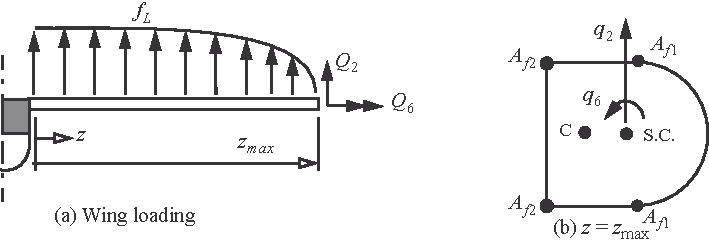
\includegraphics{Figure_6-12.pdf}}
\caption{(a) Wing spanwise airload intensity and fictitious actions $Q_{\textbf{2}}$ and $Q_{\textbf{6}}$ of example~\ref{ex6.6}. (b) Wing tip cross section and the corresponding generalized displacements $q_{\textbf{2}}$ and $q_{\textbf{6}}$.}\label{fig6.12}
\end{figure}



Numerical data for the cross-sectional dimensions are listed in table~\ref{tab6.3}.
The material is an aluminium alloy with a Young's modulus $E=10.5 \times 10^{3}~\mathrm{ksi}$, a shear modulus $G=4.0 \times 10^{3}~\mathrm{ksi}$, and with a yield strength $\sigma_{\text {yield }}=44~\mathrm{ksi}$. Additional cross-sectional properties computed from example~\ref{ex3.4} on page~\pageref{ex3.4}  are listed in table~\ref{tab6.4}.

\begin{figure}[!h]
\centerline{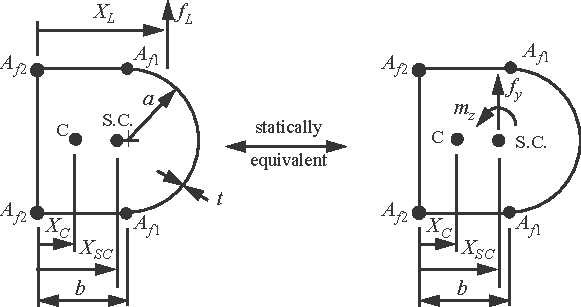
\includegraphics{Figure_6-13.pdf}}
\caption{Example~\ref{ex6.6}: Typical cross section of the uniform spar.}\label{fig6.13}
\end{figure}

\begin{table}[!h]%T3
\processtable{Cross-sectional data for the wing spar\label{tab6.3}}{%
\begin{tabular}{@{}ll|ll@{}}
\toprule
\multicolumn{4}{c}{\textbf{Dimensional data of the cross section}}\\
\toprule\\[-15.5pt]
& & \\[-6pt]
$A_{f1}$, stringer 1 flange area &0.30 in.$^2$ &$b$, length horizontal web &7.0 in. \\
$A_{f2}$, stringer 2 flange area &0.70 in.$^2$ &$t$, wall thickness &0.030 in. \\
$a$, nose web radius &6.0 in &$X_L$, location of the airload &10.0 in.\\[-3pt]
& & \\[-3.5pt]
\botrule
\end{tabular}}{}
\bigskip
\end{table}

\begin{table}[!h]%T4
\processtable{Data from example~\ref{ex3.4}\label{tab6.4}}{%
\begin{tabular}{@{}p{12pc}lp{13.8pc}l@{}}
\toprule
\textit{A}, area of the cross section &3.3455 in.$^2$ \\
$X_C$, horizontal location of the centroid &3.52367 in. &$c_{yy}$, compliance coefficient in transverse shear$^{\textrm{a}}$ &$\left(\frac{1.64758}{\textrm{in.}^{2}}\right) \frac{1}{G}$ \\
\raggedright$X_{SC}$, horizontal location of the shear center &6.39638 in. & $c_{zz}$, compliance coefficient in torsion$^{\textrm{b}}$ &$\left(\frac{0.0189201}{\text {in.}^{4}}\right) \frac{1}{G}$ \\
\raggedright$I_{xx}$, second area moment about the $x$-axis &101.619 in.$^4$ &$A_c$, area enclosed by the contour &140.549 in.$^2$ \\
\botrule
\end{tabular}}{a. \textit{Note}: From eq.~(\ref{eq5.65}) on page~\pageref{eq5.65}, $\displaystyle c_{yy}=\sum_{i\,=\,1}^4\int\limits_{0}^{(s_i)_{max}}\frac{F^2_{yi}(s_i)}{Gt}ds_i$, where the shear flow distribution functions $F_{yi}(s_i)$ are given by eqs. (\textbf{ab}) to (\textbf{ae}) in part c of example~\ref{ex3.4}.\newline
b. \textit{Note}: $c_{zz}=(GJ)^{-1}$, and from eq.~(\ref{eq3.160}) on page~\pageref{eq3.161} the torsion constant $J=(4A_c^2)/\left(\oint\frac{ds}{t}\right)$.}
\vspace*{-0.5pc}
\end{table}


\begin{enumerate}[b)]
\item[a)] Determine the statically admissible bar resultants in the spar for $0 \leq z \leq z_{\textit{max}}$.
\item[b)] Determine the generalized displacements $q_2$ and $q_6$ of the shear center at $z=z_{\textit{max}}$.
\item[c)] Tabulate the displacement $q_2$, percentage of the displacement $q_2$ due to transverse shear, and the rotation $q_6$ of part (b) for the following spar lengths: $z_{\textit{max}}=12$, 24, 60, 120, 180, 240, and 300 in.. Also, tabulate the ratio of the maximum von Mises effective stress (eq.~(\ref{eq4.31}) on page~\pageref{eq4.31}) to the yield strength in the semi-circular web, or branch 1, at $z = 0$ for the same set of spar lengths.
\end{enumerate}

\vspace*{-10pt}

\subsubsection{Solution to part (a).} The external distributed line load intensities resolved at the shear center are shown figure~\ref{fig6.13}. In terms of the specified airload $f_{y}=f_{L}$ and $m_{z}=ef_{L}$, where $e=X_{L}-X_{S C}$. The differential equation for the transverse shear force $V_y$ is given by eq.~(\ref{eq3.54}) on page~\pageref{eq3.54}. Substitute the expression for the airload to get the shear force as
\begin{equation*}
V_{y}=\int\left[-\left(\frac{2 L}{\pi z_{m a x}}\right) \sqrt{1-\left(\frac{z}{z_{m a x}}\right)^{2}}\hspace*{3pt}\right] d z=\left(\frac{L}{\pi}\right)\left[\operatorname{acos}\left(\frac{z}{z_{m a x}}\right)-\left(\frac{z}{z_{m a x}}\right) \sqrt{1-\left(\frac{z}{z_{m a x}}\right)^{2}}\hspace*{3pt}\right]+c_{1}.\tag{a}
\end{equation*}
Note that the integration is facilitated by the substitution $z / z_{\it max }=\cos \theta$, and using trigonometric identities. The constant of integration $c_1$ is determined by the boundary condition $V_{y}(z_{\it max})=Q_{2}$. Hence $c_{1}=Q_{2}$, and the final result for the shear force is
\begin{equation*}
V_{y}=\left(\frac{L}{\pi}\right)\left[\text{acos}\left(\frac{z}{z_{\it max }}\right)-\left(\frac{z}{z_{\it max }}\right) \sqrt{1-\left(\frac{z}{z_{\it max }}\right)^{2}}\hspace*{3pt}\right]+Q_{2}.\tag{b}
\end{equation*}
The shear force at the root for $Q_2 = 0$ is $V_{y}(0)|_{Q_{2}\,=\,0}=L / 2$.

The bending moment $M_x$ is determined by eq.~(\ref{eq3.55}) on page~\pageref{eq3.55}. Substitute the result for the shear force $V_y$ into eq.~(\ref{eq3.55}) to find
\[
M_{x}=\int\left\{\left(\frac{L}{\pi}\right)\left[\operatorname{acos}\left(\frac{z}{z_{\it max }}\right)-\left(\frac{z}{z_{\it max }}\right) \sqrt{1-\left(\frac{z}{z_{\it max }}\right)^{2}}\right]+Q_{2}\right\} d z.
\]
Again, the integration for $M_x$ is facilitated by the substitution $z/z_{\it max}=\cos \theta$, and using trigonometric identities to get
\begin{equation*}
M_{x}=\left(\frac{L z_{\it max}}{\pi}\right)\left[-\sqrt{1-\left(\frac{z}{z_{\it max }}\right)^{2}}+\frac{1}{3}\left[1-\left(\frac{z}{z_{\it max }}\right)^{2}\right]^{3 / 2}+\left(\frac{z}{z_{\it max }}\right) \operatorname{acos}\left(\frac{z}{z_{\it max }}\right)\right]+Q_{2} z+c_{2}.\tag{c}
\end{equation*}
The constant of integration $c_2$ is determined by the boundary condition $M_{x}\left(z_{max}\right)=0$. Hence $c_{2}=-z_{\it max } Q_{2}$, and the final result for the bending moment is
\begin{equation*}
M_{x}=\left(\frac{L z_{\it max }}{\pi}\right)\left[-\sqrt{1-\left(\frac{z}{z_{\it max }}\right)^{2}}+\frac{1}{3}\left[1-\left(\frac{z}{z_{\it max }}\right)^{2}\right]^{3 / 2}+\left(\frac{z}{z_{\it max }}\right) \operatorname{acos}\left(\frac{z}{z_{\it max }}\right)\right]-Q_{2}\left(z_{\it max }-z\right).\tag{d}
\end{equation*}
The bending moment at the root of the spar for $Q_2 = 0$ is $\left.M_{x}(0)\right|_{Q_{2}=0}=\frac{-2 L z_{m a x}}{3 \pi}$.

From eq.~(\ref{eq3.61}) on page~\pageref{eq3.61}, and that ${m}_{z}=e f_{L}$, we can express the torque $M_z$ as
\begin{equation*}
\frac{d M_{z}}{d z}=-m_{z}=-e f_{L}.\tag{e}
\end{equation*}
Hence,
\begin{equation*}
M_{z}=-e \int \!\!\frac{2 L}{\pi z_{\it max }} \sqrt{1-\left(\frac{z}{z_{\it max }}\right)^{2}} d z+c_{3}=-e \frac{L}{\pi}\left\{\left(\frac{z}{z_{\it max }}\right) \sqrt{1-\left(\frac{z}{z_{\it max }}\right)^{2}}+\operatorname{asin}\left(\frac{z}{z_{\it max }}\right)\right\}+c_{3}.\tag{f}
\end{equation*}
The constant of integration $c$3 is determined from the boundary condition $M_{z}\left(z_{\it max }\right)=Q_{6}$, which yields $c_{3}=e \frac{L}{2}+Q_{6}$. The final result for the torque is
\begin{equation*}
M_{z}=\frac{e L}{2}-\frac{e L}{\pi}\left[\left(\frac{z}{z_{m a x}}\right) \sqrt{1-\left(\frac{z}{z_{m a x}}\right)^{2}}+\operatorname{asin}\left(\frac{z}{z_{\it max }}\right)\right]+Q_{6}.\tag{g}
\end{equation*}
The torque at the root of the spar for $Q_6 = 0$ is $\left.M_{z}(0)\right|_{Q_{6}\,=\,0}=e L / 2$. We have determined the statically admissible shear force $V_y$, bending moment $M_x$, and torque $M_z$ in the wing spar in terms of the distributed airload, external force $Q_2$, and external torque $Q_6$.

\subsubsection{Solution to part (b).} From eqs. (\ref{eq5.84}) and (\ref{eq5.85}) on page~\pageref{eq5.84}, the total complementary strain energy for the bar in this example is
\begin{equation*}
U^{*}=\frac{1}{2} \int_{0}^{z_{\it max}}\left(\frac{M_{x}^{2}}{E I_{x x}}+c_{y y} V_{y}^{2}+c_{z z} M_{z}^{2}\right) d z.\tag{h}
\end{equation*}
Castigliano's second theorem for the vertical displacement of the shear center is
\begin{equation*}
q_{2}=\left.\frac{\partial U^{*}}{\partial Q_{2}}\right|_{Q_{2}\,=\,Q_{6}\,=\,0}=\left.\int_{0}^{z_{\it max }}\left[\frac{M_{x}}{E I_{x x}} \frac{\partial M_{x}}{\partial Q_{2}}+c_{y y} V_{y} \frac{\partial V_{y}}{\partial Q_{2}}+c_{z z} M_{z} \frac{\partial M_{z}}{\partial Q_{2}}\right] d z\right|_{Q_{2}\,=\,Q_{6}\,=\,0}.\tag{i}
\end{equation*}
\vspace*{5pt}
\clearpage

\noindent Note that the torque is independent of force $Q_2$, so that $\partial M_{z}/\partial Q_{2}=0$. Let $q_{2}=q_{2 m}+q_{2 v}$, where $q_{2 m}$ is the portion of the displacement due to bending moment $M_x$ and $q_{2 v}$ is the portion due to transverse shear force $V_y$.
\begin{equation*}
q_{2 m}=\left.\int_{0}^{z_{\it max }}\left[\frac{M_{x}}{E I_{x x}} \frac{\partial M_{x}}{\partial Q_{2}}\right] d z\right|_{Q_{2}\,=\,Q_{6}\,=\,0}=\left.\frac{1}{E I_{x x}} \int_{0}^{z_{\it max }} M_{x}\left[-\left(z_{\it max }-z\right)\right] d z\right|_{Q_{2}\,=\,Q_{6}\,=\,0}.\tag{j}
\end{equation*}
Substitute eq.~(\textbf{d}) for $M_x$ with $Q_2 = 0$ into eq.~(\textbf{j}), and perform the integration to get
\begin{equation*}
q_{2 m}=\frac{L(-32+45 \pi) z_{\it max }^{3}}{720 E I_{x x} \pi}.\tag{k}
\end{equation*}
The portion of the displacement due to transverse shear force $V_y$ is
\begin{align*}
q_{2 v}&=\left.\int_{0}^{z_{\it max }}\left[c_{y y} V_{y} \frac{\partial V_{y}}{\partial Q_{2}}\right] d z\right|_{Q_{2}\,=\,Q_{6}\,=\,0}=c_{y y} \int_{0}^{z_{\it max }}\left\{\left(\frac{L}{\pi}\right)\left[\operatorname{acos}\left(\frac{z}{z_{\it max }}\right)-\left(\frac{z}{z_{\it max }}\right) \sqrt{1-\left(\frac{z}{z_{\it max }}\right)^{2}}\right]\right\}\{1\} d z\nonumber\\
&=\frac{2 c_{y y} L z_{\it max }}{3 \pi}.\tag{l}
\end{align*}
Add eqs.~(\textbf{k}) and (\textbf{l}) to get the total vertical displacement at the shear center as
\begin{equation*}
q_{2}=\frac{L(-32+45 \pi) z_{\it max }^{3}}{720 E I_{x x} \pi}+\frac{2 c_{y y} L z_{m a x}}{3 \pi}.\tag{m}
\end{equation*}

Castigliano's second theorem for the rotation of the cross-section at $z=z_{\it max}$ about the shear center is
\begin{equation*}
q_{6}=\left.\frac{\partial U^{*}}{\partial Q_{6}}\right|_{Q_{2}\,=\,Q_{6}\,=\,0}=\left.\int_{0}^{z_{\it max }}\left[\frac{1}{E I_{x x}} M_{x} \frac{\partial M_{x}}{\partial Q_{6}}+c_{y y} V_{y} \frac{\partial V_{y}}{\partial Q_{6}}+c_{z z} M_{z} \frac{\partial M_{z}}{\partial Q_{6}}\right] d z\right|_{Q_{2}\,=\,Q_{6}\,=\,0}.\tag{n}
\end{equation*}
The bending moment $M_x$ and transverse shear force $V_y$ are independent of the external torque $Q_6$. Hence,
\begin{equation*}
q_{6}=\left.\frac{\partial U^{*}}{\partial Q_{6}}\right|_{Q_{2}\,=\,Q_{6}\,=\,0}=c_{z z} \int_{0}^{z_{\it max }}\left\{\frac{e L}{2}-\frac{e L}{\pi}\left[\left(\frac{z}{z_{\it max }}\right) \sqrt{1-\left(\frac{z}{z_{\it max }}\right)^{2}}+\operatorname{asin}\left(\frac{z}{z_{\it max }}\right)\right]\right\}[1] d z.\tag{o}
\end{equation*}
The integration of eq. (\textbf{o}) yields
\begin{equation*}
q_{6}=\frac{2 c_{z z} e L z_{\it max }}{3 \pi}.\tag{p}
\end{equation*}

\subsubsection{Solution to part (c).} Numerical evaluation of the displacements yields
\begin{equation*}
q_{2 m}=\left(\frac{5.438 \times 10^{-7}}{\text {in.}^{2}}\right) z_{\it max}^{3} \quad q_{2 v}=(1.0489 \times 10^{-3}) z_{\it max } \quad q_{6}=(4.3905 \times 10^{-5} \text { in.}^{-1}) z_{\it max}.\tag{q}
\end{equation*}

\vspace*{-1pc}

The expression for the shear flow is given by eq.~(\ref{eq3.163}) on page~\pageref{eq3.163}. At the root cross section the equation for the shear flow reduces to
\begin{equation*}
q(s, 0)=M_{z}(0) /\left(2 A_{c}\right)-F_{y}(s) V_{y}(0).\tag{r}
\end{equation*}

\vspace*{-1pc}\pagebreak

\noindent The torque results in a spatially uniform component to the shear flow around the contour equal to
\begin{equation*}
q_{t}=M_{z}(0) /\left(2 A_{c}\right)=76.9188~\mathrm{lb} / \mathrm{in}.\,.\tag{s}
\end{equation*}
(Refer to eq.~(\ref{eq3.165}) on p.~\pageref{eq3.165}). The total shear flow in each branch is
\begin{equation*}
q_{i}\left(s_{i}, 0\right)=76.9188~\mathrm{lb}/\text{in. }-F_{y i}\left(s_{i}\right)(6000.0 \text { lb.}) \quad i=1,2,3,4,\tag{t}
\end{equation*}
where the contour coordinates $s_i$ are shown in figure~\ref{fig3.24}(b) on page~\pageref{fig3.24}, and the shear flow distribution functions $F_{y i}\left(s_{i}\right)$ are given by eqs.~(\textbf{ab}) to (\textbf{ae}) in part c of example~\ref{ex3.4}. The shear stress distribution along the contour in each branch is given by
\begin{equation*}
\sigma_{z s i}\left(s_{i}, 0\right)=[q_{i}(s_{i}, 0)] / t \quad i=1,2,3,4.\tag{u}
\end{equation*}
In this example $I_{x y}=n_{x}=n_{y}=0$ and $k=1$ in the axial normal stress given by eq.~(\ref{eq4.6}) on page~\pageref{eq4.6}. For no change in temperature and $N=M_{y}=0$, the axial normal stress eq.~(\ref{eq4.6}) at the root cross section in each branch reduces to
\begin{equation*}
\sigma_{z i}\left(s_{i}, 0\right)=\frac{M_{x}(0) y_{i}\left(s_{i}\right)}{I_{x x}}=\left[\left(-25.0591 \frac{\mathrm{lb} .}{\mathrm{in.}^{4}}\right) z_{\it max }\right] y_{i}\left(s_{i}\right) \quad i=1,2,3,4.\tag{v}
\end{equation*}
The parametric equations for the $y$-coordinates of the contour in each branch are
\begin{equation*}
y_{1}\left(s_{1}\right)=-a \cos \left(s_{1} / a\right) \quad y_{2}=a \quad y_{3}\left(s_{3}\right)=a-s_{3} \quad y_{4}=-a.
\tag{w}
\end{equation*}
(Refer to figure~\ref{fig3.24} on page~\pageref{fig3.24}.) From eq.~(\ref{eq4.31}) the von Mises effective stress is
\begin{equation*}
\left(\sigma_{\text {Mises }}\right)_{i}=\sqrt{\left[\sigma_{z i}\left(s_{i}, 0\right)\right]^{2}+3\left[\sigma_{z s i}\left(s_{i}, 0\right)\right]^{2}} \quad i=1,2,3,4.\tag{x}
\end{equation*}
The von Mises effective stress normalized by the yield strength is plotted with respect to the contour coordinate for $z_{\it max} = 60$ inches in figure~\ref{fig6.14}. As shown in the figure the maximum normalized effective stress is 0.383 at $s = 4.696$ in. in branch 1. In terms of an angular measurement in the semi-circular branch 1, we note the location as $s_{1} / a=(4.696 / 6)\left(180^{\circ} / \pi\right)=44.8^{\circ}$. For the other values of $z_{\it max}$, the maximum value of the von Mises stress also occurs in branch 1 but at different angular locations. Discontinuities in the von Mises stress with respect to the contour coordinate are a result of the jumps in the shear flow across the stringers. (Refer to eq.~(\ref{eq3.135}) on p.~\pageref{eq3.135}).


\processfigure{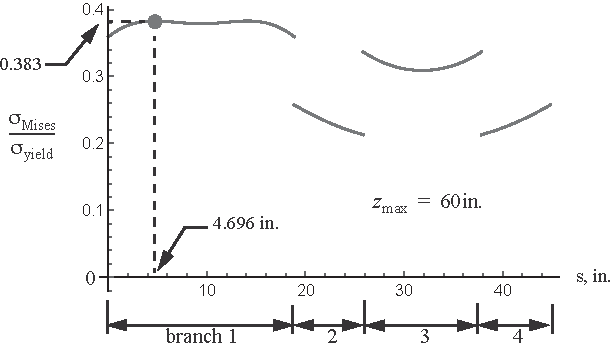
\includegraphics{Figure_6-14.pdf}
}
{\caption{Normalized von Mises effective stress plotted with respect to the contour\break coordinate s at the root cross section of the spar.}\label{fig6.14}}

Numerical results are listed in table~\ref{tab6.5}.
\vspace*{5pt}
\clearpage

\begin{table}%T5
\processtable{Wing tip displacements and wing root stresses as a function of the span\label{tab6.5}}
{\begin{tabular}{@{}lccccc@{}}
\toprule
&\multicolumn{3}{c}{\colhead{Wing tip}} &\multicolumn{2}{c}{\colhead{Wing root}}\\[-5pt]
&\multicolumn{3}{c}{\hrulefill} &\multicolumn{2}{c}{\hrulefill} \\
\colhead{$z_{\textbf{\textit{max}}}, \text { in.}$} & \colhead{$\textbf{\textit{q}}_{\textbf{2}} \text {, in. }$} & \colhead{$\textbf{\textit{q}}_{\textbf{2}\textbf{\textit{v}}} / \textbf{\textit{q}}_{\textbf{2}}$,\%} & \colhead{$\textbf{\textit{q}}_{\textbf{6}}, \text { deg. }$} & \colhead{$\boldsymbol{\sigma}_{\textbf{Mises}} / \boldsymbol{\sigma}_{\textbf{yield}}$} & \colhead{$\textbf{\textit{s}}_{\textbf{1}} / \textbf{a}$, deg.} \\
\midrule
12. &0.0135 &93.1\phantom{.} &0.0298 &0.379 &90.0\phantom{.} \\
24. &0.0327 &77.0\phantom{.} &0.0597 &0.379 &90.0\phantom{.} \\
60. &0.180\phantom{0} &34.9\phantom{.} &0.149\phantom{0} &0.383 &44.8\phantom{.} \\
120. &1.066\phantom{0} &11.8\phantom{.} &0.298\phantom{0} &0.509 &\phantom{0.}8.82 \\
180. &3.360\phantom{0} &\phantom{0.}5.62 &0.448\phantom{0} &0.683 &\phantom{0.}3.81 \\
240. &7.77\phantom{00} &\phantom{0.}3.29 &0.597\phantom{0} &0.872 &\phantom{0.}2.13 \\
300. &15.0\phantom{00} &\phantom{0.}2.10 &0.746\phantom{0} &1.07\phantom{0} &\phantom{0.}1.36 \\
\botrule
\end{tabular}}{}
\vspace*{-1pc}
\end{table}


\noindent Note that as the length of the spar increases the percentage of the vertical displacement at the tip due to transverse shear decreases and the von Mises effective stress increases. At $z_{\it max} = 300$ in. the von Mises stress exceeds the yield strength of the material indicating failure by material yielding.
\end{example*}

\vspace*{-1pc}

\section{Coplanar frames}\label{sec6.3}
Frames are also skeletal structures composed of slender bars that can transmit axial, bending, and transverse shear loads. The bars act as beams with a superimposed axial load. Joints in a frame are usually assumed rigid, which means that the rotation of all bars connected to the joint are the same. Moments can be transferred through a rigid joint, but not a hinge joint, nor ball-and-socket joint. A frame structure may also contain some hinge joints.

\begin{wrapfigure}[12]{R}{153.16pt}
\vspace{12pt}
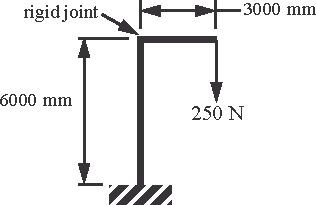
\includegraphics{Figure_6-15.pdf}
\caption{Tubular post \label{fig6.15}}
\end{wrapfigure}

\begin{example}[A frame of two tubular bars]\label{ex6.7}The tubular post shown in figure~\ref{fig6.15} supports a load of 250~N at the free end. The diameter of the cross-sectional contour is 100~mm and the wall thickness is 3~mm. The material is steel with modulus of elasticity of 206,000 N/mm$^2$ and a Poisson's ratio of 0.3. Each bar of the frame has the same uniform geometric cross section along its length. Find the vertical and horizontal displacement of the free end.


\subsubsection{Solution.} We use Castigliano's second theorem to determine the displacements of the free end for this statically determinate structure. A horizontal force $Q$ is introduced at the free end so that the horizontal displacement can be computed from the theorem. Also, let $P = 250$~N. The complementary strain energy is determined from eqs. (\ref{eq5.84}) and (\ref{eq5.85}). Since there is no change in temperature nor torsion, the complementary strain energy is
\begin{equation*}
U^{*}=\sum_{{\it bars}}\int_{0}^{L}\left[\frac{N^{2}}{2 E A}+\frac{M_{x}^{2}}{2 E I_{x x}}+\frac{1}{2} c_{y y} V_{y}^{2}\right] d z.\tag{a}
\end{equation*}
Let $u_{P}$ denote the displacement corresponding to force $P$, and let $u_{Q}$ denote the displacement corresponding to force $Q$. These displacements are given by\pagebreak
\begin{equation*}
u_{P}=\left.\frac{\partial U^{*}}{\partial P}\right|_{P\,=\,250, Q\,=\,0} \quad u_{Q}=\left.\frac{\partial U^{*}}{\partial Q}\right|_{P\,=\,250, Q\,=\,0}.\tag{b}
\end{equation*}
The coordinate system in each bar is shown in figure~\ref{fig6.16}(a), the free body diagram for the vertical bar in figure~\ref{fig6.16}(b), and the free body diagram of the horizontal bar is shown in figure~\ref{fig6.16}(c) The partial derivatives of the complementary strain energy for the frame with respect to the external loads are

\processfigure{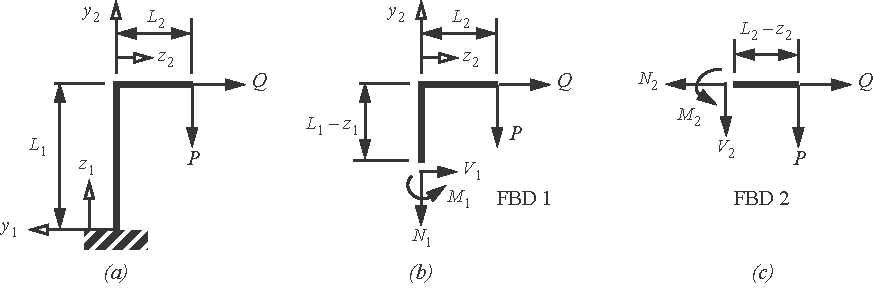
\includegraphics{Figure_6-16.pdf}
}
{\caption{(a) Coordinates in each bar. (b) FBD of vertical bar. (c) FBD of horizontal bar.}\label{fig6.16}}

\vspace*{-1.5pc}

\begin{align*}
\frac{\partial U^{*}}{\partial P}&=\int_{0}^{L_{1}}\left(\frac{N_{1}}{E A} \frac{\partial N_{1}}{\partial P}+\frac{M_{1}}{E I_{x x}} \frac{\partial M_{1}}{\partial P}+c_{y y} V_{1} \frac{\partial V_{1}}{\partial P}\right) d z_{1}+\int_{0}^{L_{2}}\left(\frac{N_{2}}{E A} \frac{\partial N_{2}}{\partial P}+\frac{M_{2}}{E I_{x x}} \frac{\partial M_{2}}{\partial P}+c_{y y} V_{2} \frac{\partial V_{2}}{\partial P}\right) d z_{2},\ \text{and}\tag{c}\\
\frac{\partial U^{*}}{\partial Q}&=\int_{0}^{L_{1}}\left(\frac{N_{1}}{E A} \frac{\partial N_{1}}{\partial Q}+\frac{M_{1}}{E I_{x x}} \frac{\partial M_{1}}{\partial Q}+c_{y y} V_{1} \frac{\partial V_{1}}{\partial Q}\right) d z_{1}+\int_{0}^{L_{2}}\left(\frac{N_{2}}{E A} \frac{\partial N_{2}}{\partial Q}+\frac{M_{2}}{E I_{x x}} \frac{\partial M_{2}}{\partial Q}+c_{y y} V_{2} \frac{\partial V_{2}}{\partial Q}\right) d z_{2},\tag{d}
\end{align*}
\noindent where $L_{1}=6000\,\mathrm{mm}$ and $L_{2}=3000\,\mathrm{mm}$. Equilibrium determines the internal actions $N, V, M$ in each bar. The results are
\begin{align*}
&N_{1}=-P \quad V_{1}=-Q \quad M_{1}=L_{2} P+\left(L_{1}-z_{1}\right) Q \quad z_{1} \in\left[0, L_{1}\right],\ \text{and}&\tag{e}\\
&N_{2}=Q \quad V_{2}=-P \quad M_{2}=\left(L_{2}-z_{2}\right) P \quad z_{2} \in\left[0, L_{2}\right].&\tag{f}
\end{align*}
Evaluating the partial derivatives based on equilibrium conditions we get
\begin{align*}
\frac{\partial U^{*}}{\partial P}=& \int_{0}^{L_{1}}\left[\frac{(-P)}{E A}(-1)+\frac{\left(L_{2} P+\left(L_{1}-z_{1}\right) Q\right)}{E I_{x x}}\left(L_{2}\right)+c_{y y}(-Q)(0)\right] d z_{1}\\
& + \int_{0}^{L_{2}}\left(\frac{(Q)}{E A}(0)+\frac{\left(L_{2}-z_{2}\right) P}{E I_{x x}}\left(L_{2}-z_{2}\right)+c_{y y}(-P)(-1)\right) d z_{2},\ \text{and}\tag{g}\\
\frac{\partial U^{*}}{\partial Q}=&\int_{0}^{L_{1}} \left[\frac{(-P)}{E A}(0)+\frac{\left(L_{2} P+\left(L_{1}-z_{1}\right) Q\right)}{E I_{x x}}\left(L_{1}-z_{1}\right)+c_{y y}(-Q)(-1)\right] d z_{1} \\
&+ \int_{0}^{L_{2}}\left[\frac{(Q)}{E A}(1)+\frac{\left(L_{2}-z_{2}\right) P}{E I_{x x}}(0)+c_{y y}(-P)(0)\right] d z_{2}.\tag{h}
\end{align*}
The displacements can now be computed from the expressions for the partial derivatives as
\begin{gather*}
u_{p}=\int_{0}^{L_{1}}\left[\frac{P}{E A}+\frac{L_{2}^{2} P}{E I_{x x}}\right] d z_{1}+\left.\int_{0}^{L_{2}}\left[\frac{\left(L_{2}-z_{2}\right)^{2} P}{E I_{x x}}+c_{y y} P\right] d z_{2}\right|_{P=250}=\frac{L_{1} P}{E A}+\underbrace{\frac{L_{1} L_{2}^{2} P}{E I_{x x}}+\frac{L_{2}^{3} P}{3 E I_{x x}}}_{\text {bending }}+\left.c_{y y} L_{2} P\right|_{P=250}\tag{i}\\
u_{Q}=\left.\frac{\partial U^{*}}{\partial Q}\right|_{P=250, Q=0}=\left.\int_{0}^{L_{1}}\left[\frac{\left(L_{2} P\right)}{E I_{x x}}\left(L_{1}-z_{1}\right)\right] d z_{1}\right|_{P=250}=\left.\frac{L_{1}^{2} L_{2}}{2 E I_{x x}}\right|_{P=250}.\tag{j}
\end{gather*}
The formulas for the section properties are given in example \ref{ex6.4} on page \pageref{ex6.4}. For $a=50\,\mathrm{mm}$ and $t=3\,\mathrm{mm}$ we get
\begin{equation*}
A=300 \pi~\mathrm{mm}^{2} \quad c_{y y}=\frac{1}{G\left(150 \pi~\mathrm{mm}^{2}\right)} \quad I_{x x}=375000 \pi~\mathrm{mm}^{4}.\tag{k}
\end{equation*}
For an isotropic material the shear modulus is computed from $G=E /[2(1+v)]$, which evaluates to $G=79231\,\mathrm{N} / \mathrm{mm}^{2}$. Numerical evaluation of the displacements gives
\begin{align*}
&u_{P}=\frac{(6000) 250}{(206000)(300 \pi)}+\frac{(6000)(3000)^{2} 250}{(206000)(375000 \pi)}+\frac{(3000)^{3} 250}{3(206000)(375000 \pi)}+\frac{(3000) 250}{(79231)(150 \pi)},\tag{l}\\
&u_{P}=0.0077259681+55.62697+9.2711617+0.020087459=64.925946\,\mathrm{mm},\ \mbox{and}\tag{m}\\
&u_{Q}=\frac{(6000)^{2}(3000) 250}{2(206000)(375000 \pi)}=55.62697\,\mathrm{mm}.\tag{n}
\end{align*}
Note that the contribution to the displacement $u_{p}$ due to bending is $55.62697+9.2711617=64.898132\,\mathrm{mm}$, which is $\left(\frac{64.898132}{64.925946}\right) 100=99.957161 \%$ of the total displacement. \textbf{As a general rule the deflections of frames composed of slender bars is dominated by bending, and the contributions due to axial stretching and transverse shear deformations to the deflections can be neglected.}
\end{example}

\section{Castigliano's second theorem and statically indeterminate structures}\label{sec6.4}

A statically indeterminate structure is one in which the number of unknown forces exceeds the number of independent equations of static equilibrium. The excess forces are called redundants. By removing supports and/or members in a statically indeterminate structure equal to the number of redundants, a stable statically base structure can be obtained. To determine the redundants, we can imposed displacement compatibility using Castigliano's second theorem. A stable statically determinate base structure is capable of resisting the external loads. Removing a support reaction or a member in statically determinate structure renders it unstable---it is not capable of resisting external loads and it is classified as moving mechanical system (i.e., either a mechanism or linkage).

Consider a coplanar truss which consists of straight bars connected by smooth hinge joints with the external loads applied only to the joints. As discussed in example~\ref{ex6.3} on page~\pageref{ex6.3}, a truss is statically determinate if $m=2 j-r$ and statically indeterminate if $m>2 j-r$, where $m$ denotes the number of bars or members, $j$ the number of joints, and $r$ denotes the number of reaction forces at the supports. Even statically determinate trusses can be unstable if the members are not arranged properly. Statical determinacy is a necessary condition for stability, not a sufficient condition. Each truss must be examined individually to determine stability. For the truss shown in part (a) of figure~\ref{fig6.17}, $m = 9$, $r = 4$, and $j= 6$, so it is statically indeterminate. If the upper left support is removed and replaced with a horizontal force $Q$, then a statically determinate base structure results as shown in part (b) of figure~\ref{fig6.17}. The force $Q$ is the redundant and it is treated as an external load on the base structure. Equilibrium of the base structure determines the internal bar forces in terms of external forces $P$ and $Q$. The solution to the truss in part (a) is effected by imposing the displacement corresponding to force $Q$ to vanish via Castigliano's second theorem (i.e., $q=\partial U^{*} / \partial Q=0$). This displacement compatibility condition determines the redundant $Q$.

\begin{figure}
\centerline{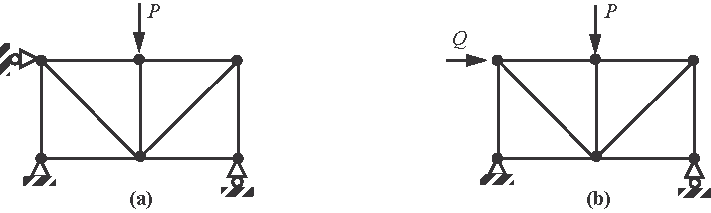
\includegraphics{Figure_6-17.pdf}}
\caption{A singly redundant truss (a), and its stable statically determinate base structure (b).}\label{fig6.17}
\end{figure}

\begin{example}[Statically indeterminate truss]\label{ex6.8}Consider the truss shown in part (a) of figure~\ref{fig6.18}. The horizontal bars and the vertical bars have a length denoted by \textit{L}, and each bar has the same elastic modulus \textit{E} and same cross-sectional area \textit{A}. For this truss $m = 6$, $r = 3$, and $j= 4$. So the truss is statically indeterminate. Note that this truss is statically determinate externally, but is statically indeterminate internally. Determine the bar forces in terms of the external applied load \textit{P}.

\processfigure{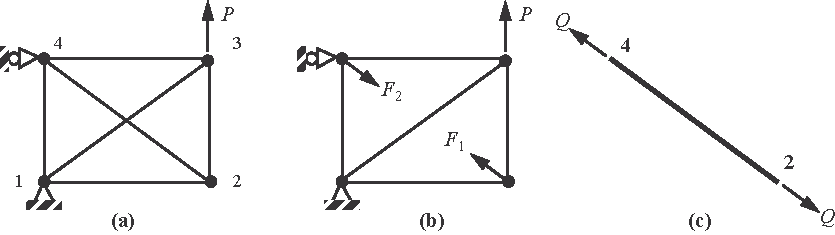
\includegraphics{Figure_6-18.pdf}
}
{\caption{(a) Statically indeterminate truss. (b) Statically determinant base structure with bar
2-4 replaced by forces $\textbf{\textit{F}}_{\textbf{1}}$ and $\textbf{\textit{F}}_{\textbf{2}}$. (c) Bar 2-4 subject to equal and opposite forces.\label{fig6.18}}}

\subsubsection{Solution.} Consider a statically determinate truss with bar 2-4 removed, and a force $F_1$ acting at joint 2 and a force $F_2$ acting at joint 4 as shown in figure~\ref{fig6.18}(b). These forces are oppositely directed along a line action coinciding with the removed bar 2-4. Let the complementary strain energy for this statically determinate, five-bar truss be denoted by $\hat{U}^{*}$. We employ Castigliano's second theorem to determine the displacement $u_1$ corresponding to force $F_1$ and displacement $u_2$ corresponding to $F_2$. That is,\setcounter{equation}{0}\def\theequation{\alph{equation}}
\begin{align}
u_{i}=\frac{\partial \hat{U}^{*}}{\partial F_{i}}=\frac{1}{E A}\left[L N_{12} \frac{\partial N_{12}}{\partial F_{i}}+\sqrt{2} L N_{13} \frac{\partial N_{13}}{\partial F_{i}}+L N_{14} \frac{\partial N_{14}}{\partial F_{i}}+L N_{23} \frac{\partial N_{23}}{\partial F_{i}}+L N_{34} \frac{\partial N_{34}}{\partial F_{i}}\right] \quad i=1,2.
\end{align}
The bar forces are determined by joint equilibrium, and the results are shown in table~\ref{tab6.6}. Bar forces are assumed positive in tension.

\begin{table}[!h]
\processtable{Terms in eq. (a) for Castigliano's second theorem\label{tab6.6}}
{\begin{tabular}{@{}llllll|l@{}}
\toprule\\[-15.5pt]
 & & & & & & \\[-5pt]
 & & & & & & \colhead{$F_{1}=F_{2}=Q$}\\[3pt]
\colhead{Bar} &\colhead{Length \textit{L}} &\colhead{Axial force \textit{N}} &\colhead{$\partial N / \partial F_{1}$} & \colhead{$L N \frac{\partial N}{\partial F_{1}}$} & \colhead{$L N \frac{\partial N}{\partial F_{2}}$} & \colhead{$L N \frac{\partial N}{\partial Q}$} \\
 & & & & & & \\[-8pt]
\midrule\\[-15pt]
 & & & & & & \\[-4.5pt]
1-2 &$L$ &$-F_{1}/\sqrt{2}$ &$-1/\sqrt{2}$ &$L F_{1} / 2$ &0 &$L Q / 2$ \\
1-3 &$\sqrt{2} L$ &$F_{1}+\sqrt{2} P$ &1 &$\sqrt{2} L F_{1}+2 L P$ &0 &$\sqrt{2} L Q+2 L P$ \\
1-4 &$L$  &$-F_{2}/\sqrt{2}$ &0 &0 &$\left(L F_{2}\right) / 2$ &$(L Q)/2$ \\
2-3 &$L$ &$-F_{1} / \sqrt{2}$ &$-1/\sqrt{2}$ &$L F_{1} / 2$ &0 &$L Q/2$ \\
3-4 &$L$ &$-F_{1} / \sqrt{2}-P$ &$-1 / \sqrt{2}$ &$L F_{1} / 2+L P / \sqrt{2}$ &0 &$L Q/2+L P/\sqrt{2}$ \\[-4.5pt]
 & & & & & & \\[-4pt]
\botrule
\end{tabular}}{}
\vspace*{-0.5pc}
\end{table}

\noindent The sum of elements in column five divided by the product \textit{EA} determines displacement $u_1$, and the sum of column six divided by \textit{EA} determines $u_2$. Simplifying the results leads to
\begin{align}
u_{1}=\frac{L}{E A}\left[\frac{3+2 \sqrt{2}}{2}\right] F_{1}+\frac{L}{E A}\left[\frac{4+\sqrt{2}}{2}\right] P\ \text{and}\ u_{2}=\frac{L}{2 E A} F_{2}.
\end{align}
The relative inward displacement between joints 2 and joint 4 is given by the sum $u_{1}+u_{2}$. For equal and opposite forces we set $F_{1}=F_{2}=Q$, and then the relative inward displacement reduces to
\begin{align}
\Delta_{1 / 2}=u_{1}+\left.u_{2}\right|_{F_{1}\,=\,F_{2}\,=\,Q}=\frac{L}{E A}[2+\sqrt{2}] Q+\frac{L}{E A}\left[\frac{4+\sqrt{2}}{2}\right] P.
\end{align}
The seventh column in the table is obtained by setting $F_{1}=F_{2}=Q$. The sum of elements in the seventh column divided by \textit{EA} is derivative of $\hat{U}^{*}$ with respect to \textit{Q}; i.e.,
\begin{align}
\frac{\partial \hat{U}^{*}}{\partial Q}=\frac{L}{E A}[2+\sqrt{2}] Q+\frac{L}{E A}\left[\frac{4+\sqrt{2}}{2}\right] P.
\end{align}
We conclude that the relative inward displacement between joints 2 and joint 4 is given by
\begin{align}
\Delta_{1 / 2}=\frac{\partial \hat{U}^*}{\partial Q}.
\end{align}

\vspace*{-1pc}

The elongation of bar 2-4 is denoted by $\Delta_{24}$ and its complementary strain energy is denoted by $U^{*}{ }_{24}$.
Hooke's law for bar 2-4 is given by eq.~(\ref{eq6.2}) on page~\pageref{eq6.2}, which for $N \rightarrow Q$ and $L \rightarrow \sqrt{2} L$ is solved for its elongation. The complementary strain energy is given by eq.~(\ref{eq5.84}) on page~\pageref{eq5.84}. These relations are
\begin{align}
\Delta_{24}=\frac{\sqrt{2} L}{E A} Q\ \text{and}\ U_{24}^{*}=\left.\frac{1}{2 E A} \int_{0}^{\sqrt{2 L}} N^{2} d z\right|_{N=Q}=\frac{\sqrt{2} L}{2 E A} Q^{2}.
\end{align}
Castigliano's second theorem is $\frac{\partial U^{*} 24}{\partial Q}=\frac{\sqrt{2} L}{E A} Q$, which is equal to the elongation. Thus, $\Delta_{24}=\frac{\partial U_{24}^{*}}{\partial Q}$.

\textbf{Geometric compatibility} of the statically indeterminate, six-bar truss requires the relative inward displacement between joints 2 and 4 equals the negative of the elongation of bar 2-4. In other words, the sum $\Delta_{1 / 2}+\Delta_{24}=0$. Hence,
\begin{align}
\Delta_{1 / 2}+\Delta_{24}=\frac{\partial \hat{U}^{*}}{\partial Q}+\frac{\partial U_{24}^{*}}{\partial Q}=\frac{\partial U^{*}}{\partial Q}=0,
\end{align}
where the total complementary strain energy of the statically indeterminate six-bar truss is $U^{*}=\hat{U}^{*}+U^{*}_{24}$. Hence, Castigliano's second theorem applied to the six-bar truss is
\begin{align}
\frac{\partial U^{*}}{\partial Q}=\underbrace{\frac{L}{E A}[2+\sqrt{2}] Q+\frac{L}{E A}\left[\frac{4+\sqrt{2}}{2}\right] P}_{\frac{\partial \hat{U}^{*}}{\partial Q}}+\underbrace{\frac{\sqrt{2} L}{E A} Q}_{\frac{\partial U^{*}{ }_{24}}{\partial Q}}=\frac{L}{E A}\{2(1+\sqrt{2}) Q+[(4+\sqrt{2}) P] / 2\}=0.
\end{align}
From eq. (\textbf{h}) we determine the redundant as
\begin{align}
Q=-\left(\frac{4+\sqrt{2}}{4(1+\sqrt{2})}\right) P=-0.56066 P.
\end{align}
Finally, the bar forces are
\begin{align}
\begin{array}{crrr}N_{1-2}=0.396447 P & N_{1-3}=0.853553 P & N_{1-4}=0.396447 P \\N_{2-3}=0.396447 P & N_{2-4}=-0.56066 P & N_{3-4}=-0.603553 P\end{array}.
\end{align}

\vspace*{-1pc}

The condition that $\partial U^{*} / \partial Q=0$ is interpreted as the relative displacement between the faces of an imaginary cut in bar 2-4 is equal to zero.
\end{example}

\vspace*{-1.5pc}

If the solution of the truss in example~\ref{ex6.8} was undertaken using Castigliano's first theorem, it would lead to five simultaneous linear equations for the unknown joint displacements $q_{3}, q_{4}, q_{5}, q_{6}$, and, $q_{8}$ in terms of the applied load $P$. (Refer to ``Coplanar trusses'' on page~\pageref{sec6.1} for the displacement numbering convention.) After solving for these simultaneous equations for the joints displacements, the elongations of each bar, $\Delta_{i-j}$, would be computed from eq.~(\ref{eq6.6}) on page~\pageref{eq6.6}. Lastly, the bar forces are determined from $N_{i-j}=(E A / L)_{i-j} \Delta_{i-j}$. Using Castigliano's second theorem for this singly redundant truss, we only had to solve one equation for the unknown redundant $Q$. The number of simultaneous equations to be solved in a statically indeterminate structure by Castigliano's second theorem is equal to the number of redundants.

\begin{example*}[King Post truss]\label{ex6.9}In this example we paraphrase the problem statement given in the text by Bruhn (1973, p.~A8.42). The structure shown in figure~\ref{fig6.19} consists of members ADC, AB, BC, and BD. Continuous member ADC is simply supported at ends A and C, has an area of 9.25 in$^2$, and a second area moment of 216 in$^4$. Members AB, BC and BD have areas of 2 in$^2$. The modulus of elasticity is the same for all members. Determine the internal actions in each member using Castigliano's second theorem.
\vspace*{10pt}
\pagebreak

\begin{wrapfigure}[10]{R}{181.80pt}
\vspace{-19pt}
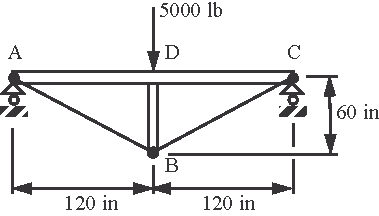
\includegraphics{Figure_6-19.pdf}
\caption{King post truss. \label{fig6.19}}
\end{wrapfigure}


\subsubsection{Solution.} This structure is statically determinant externally.
 Also, the structure, its support conditions, and the external loading are symmetric about the vertical line of action of the 5,000~lb. force. The support reactions of the truss removed from its supports at A and C are shown in figure~\ref{fig6.20}(a). Consideration of the free body diagrams of members AD, AB, and BD in figure~\ref{fig6.20}(b) leads to the conclusion that this structure is statically indeterminate internally. The redundant $Q$ is taken as the axial force in member AB. If $Q$ is known, then the forces and moments in the other members are determined by equilibrium. Neglecting the energy due to transverse shear in member ADC, the complementary strain energy is
\setcounter{equation}{0}\def\theequation{\alph{equation}}
\processfigure[!h]{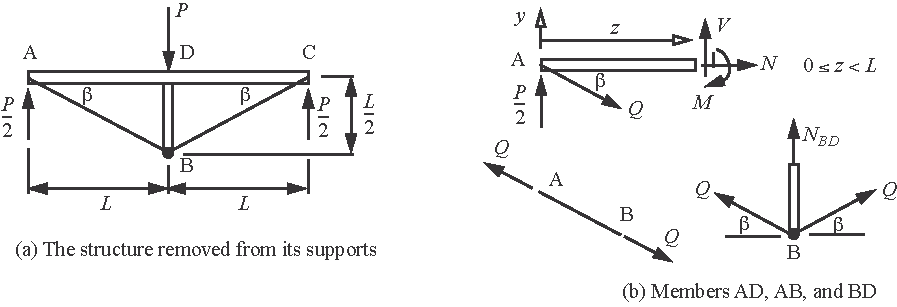
\includegraphics{Figure_6-20.pdf}}{\caption{Free body diagrams of the king post truss.\label{fig6.20}}}
\begin{align}
U^{*}=2 \int_0^L\left[\frac{N^{2}}{2 E A_{A C}}+\frac{M^{2}}{2 E I}\right] d z+2\left[\frac{L_{A B} Q^{2}}{2 E A}\right]+\frac{(L / 2) N_{B D}^{2}}{2 E A}.
\end{align}
\looseness-1Note that the complementary strain energy in members AD and AB are multiplied by two to account for the energy in members DC and BC, respectively. The compatibility condition that the relative displacement of an imaginary cut in member AB vanishes is that the derivative of the complementary energy with respect to $Q$ equals zero. Thus,
\begin{align}
0=2 \int_{0}^{L}\left\{\frac{N}{E A_{A C}}\left(\frac{\partial N}{\partial Q}\right)+\frac{M}{E I}\left(\frac{\partial M}{\partial Q}\right)\right\} d z+\frac{2 L_{A B} Q}{E A}+\frac{(L / 2) N_{B D}}{E A}\left(\frac{\partial N_{A B}}{\partial Q}\right).
\end{align}
Equilibrium equations of member AD are
\begin{align}
N+Q \cos \beta=0 \quad V+P / 2-Q \sin \beta=0 \quad M+(P / 2-Q \sin \beta) z=0 \quad 0 \leq z<L.
\end{align}
The axial equilibrium equation for member BD is
\begin{align}
N_{B D}+2 Q \sin \beta=0.
\end{align}
Substitute member axial forces and moment from the equilibrium eq. (\textbf{c}) into the compatibility condition (\textbf{b}) to get
\begin{align}
0=2 \int_{0}^{L}\left\{\frac{(-Q \cos \beta)}{E A_{A C}}(-\cos \beta)+\frac{[-(P / 2-Q \sin \beta) z]}{E I}[(\sin \beta) z]\right\} d z+\frac{2 L_{A B} Q}{E A}+\frac{(L / 2)(-2 Q \sin \beta)}{E A}(-2 \sin \beta).
\end{align}
Perform the integration in eq. (\textbf{e}) followed by the substitutions $L_{A B}=(\sqrt{5} L) / 2$, $\cos \beta=2 /(\sqrt{5})$, and $\sin \beta=1 /(\sqrt{5})$ to find
\begin{align}
0=2\left(\frac{-L^{3} P}{6 \sqrt{5} E I}+\frac{4 L Q}{5 E A_{A C}}+\frac{L^{3} Q}{15 E I}\right)+\frac{2 L Q}{5 E A}+\frac{\sqrt{5} L Q}{E A}.
\end{align}
Solve. (\textbf{f}) for the redundant \textit{Q}:
\begin{align}
Q=\frac{\sqrt{5} A A_{A C} L^{2} P}{24 A I+6 A_{A C} I+15 \sqrt{5} A_{A C} I+2 A A_{A C} L^{2}}.
\end{align}
Substitute the numerical values for the quantities on the right-hand side of eq. (\textbf{g}) to find the redundant:
\begin{align}
Q=\frac{\sqrt{5}(2)(\ref{eq9.25})\left(120^{2}\right)(5000)}{24(2)(216)+6(\ref{eq9.25})(216)+15 \sqrt{5}(\ref{eq9.25})(216)+2(2)(\ref{eq9.25})\left(120^{2}\right)}=4{,}787.18~\mathrm{lb}.
\end{align}
The axial force in member BD from eq. ({\bf d}) is
\[
N_{B D}=-2(4787.18)\left(\frac{1}{\sqrt{5}}\right)=-4281.78~\mathrm{lb}.
\]
The negative value of $N_{B D}$ means member BD is in compression. The axial force and bending moment in member AD is
\begin{align}
N=-(4787.18) 2 / \sqrt{5}=-4281.78~\mathrm{lb} . \quad M=\left(-2500+\frac{(4787.18)}{\sqrt{5}}\right) z=(-359.11~\mathrm{lb} .) z \quad 0 \leq z<120~\mathrm{in.}
\end{align}\hfill\qed
\end{example*}

\vspace*{-1pc}

\subsection{Function of a Turnbuckle}\label{sec6.4.1}

A turnbuckle is a metal coupling device consisting of an oblong piece, or barrel, internally threaded at both ends into which the corresponding sections of two threaded rods are screwed in order to form a unit that can be adjusted for tension or length. A right-hand thread is used at one end and a left-hand thread at the other end. The device either lengthens or shortens when the barrel is rotated. Each full turn of the barrel causes it to travel a distance $p$ along each screw, where $p$ is the pitch of the threads. Tightening the turnbuckle by one turn causes the rods to be drawn closer together by a distance $2p$. That is, one turn to tighten causes the device to shorten by 2p. For $n$ turns the shortening distance is $2np$, where $n$ need not be an integer. Turnbuckles are widely used in aircraft. Biplanes may use turnbuckles to adjust the tension on structural wires bracing their wings as discussed in example 6.10 below. Turnbuckles are also widely used with flexible cables in flight control systems.

\begin{example*}[Rigging biplane landing and flying wires]\label{ex6.10}An acrobatic biplane has a maximum gross weight of 1,700 lbs. and a wing span of 25 feet. The cross sections of the lower and upper wings are thin, so the wing structure is strengthened by external bracing. As shown in figure~\ref{fig6.21} the bracing consists of landing and flying wires connecting the fuselage to the wings at the interplane strut. Turnbuckles inserted in the landing and flying wires are used to pre-tension the wires by changing their length.

\processfigure{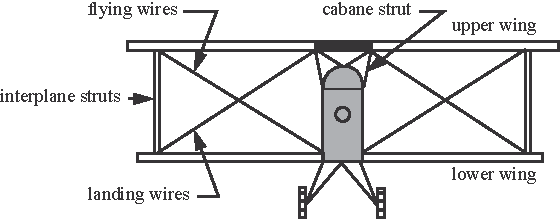
\includegraphics{Figure_6-21.pdf}}{\caption{Aerobatics biplane.\label{fig6.21}}}

We will model the structural unit consisting of the lower wing, upper wing, interplane strut, landing wires, and flying wires as shown in figure~\ref{fig6.22}(a). The left-hand wings are modeled as a pin-jointed truss.\vadjust{\vspace*{10pt}\pagebreak} Bars 1-2\break and 3-4 represent the spars in the lower wing and upper wing, respectively, and are of length $L = 10$~ft. The spars are made of Sitka spruce with a Young's modulus parallel to the grain of $1.5 \times 10^{6}$ lb./in.$^2$, and a cross-sectional area of 1.25 in.$^2$. Bar 1-3 represents the landing wire, bar 2-4 the flying wire, and the wires are made of stainless steel with a modulus of $30 \times 10^{6}$ lb./in.$^2$ Each wire has a diameter of 0.125 in. Bar 1-4 is the interplane strut of length $h$ equal to 4.3 ft., and it is assumed to be very stiff. The wings are specified to have a dihedral angle\break $\Gamma=4^{\circ}$.

Determine the number of turns in the flying wire turnbuckle $n_{F}$, and the number of turns in the landing wire turnbuckle $n_{L}$, such that the flying wire tension is 400 lb., and the dihedral is maintained at four degrees. The pitch of the turnbuckle threads is $p=1~\text {in.}/(10~\text {turns})$.


%\medskip\noindent
\subsubsection{Solution.} The structural model of the left-hand wing and bracing shown in figure~\ref{fig6.22}(a) consists of five truss bars. The turnbuckle displacements are determined from the horizontal position of the wing. Free body diagrams of joints 1 and 4 are shown in figure~\ref{fig6.22}(b). A vertical external force $Q_2$ is introduced at joint 1 so that its corresponding displacement $q_2$ can be determined in the application of Castigliano's theorem. Displacement $q_2$ is specified from the wing's required dihedral. That is $q_{2}=L \sin \Gamma$, and after its determination external force $Q_{2}$ is set to zero.

From eq.~(\ref{eq5.84}) on page~\pageref{eq5.84} the complementary energy for a homogenous truss bar subject to a uniform change in temperature is
\setcounter{equation}{0}\def\theequation{\alph{equation}}
\begin{align}
U^{*}=\frac{L}{2 E A}\left(N+N_{T}\right)^{2}.
\end{align}
To account for the displacements of the turnbuckles in Castigliano's second theorem we modify the axial temperature term in the complementary strain energy. The thermal axial force in the truss bar is obtained from eq.~(\ref{eq3.75}) on page~\pageref{eq3.75}:
\begin{align}
N_{T}=\int_{c} \beta \Delta T(s, z) t(s) d s=E A \alpha \Delta T.
\end{align}
Let the thermal strain $\alpha \Delta T$ be replaced by the initial strain induced by the turnbuckle displacement $\Delta_{T}=2 n p$ divided by the length of the bar containing the turnbuckle. That is, $\alpha \Delta T \rightarrow \Delta_{T} / L$. Then the complementary strain energy in eq. (\textbf{a}) that includes the displacement caused by the turnbuckle is
\begin{align}
U^{*}=\frac{c}{2}\left(N+\Delta_{T} / c\right)^{2},
\end{align}
where the flexibility influence coefficient $c=L /(E A)$.

\begin{figure}[!h]
\centerline{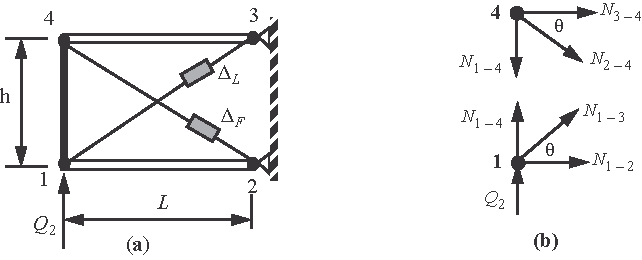
\includegraphics{Figure_6-22.pdf}}
\caption{(a) Structural model of the left-hand wing and bracing. (b) Free body diagrams.}\label{fig6.22}
\end{figure}

The interplane strut subject to force $N_{1-4}$ is assumed to be rigid. Its flexibility influence coefficients vanishes and it does not contribute the elastic complementary strain energy. The complementary strain energy is
\begin{align}
U^{*}=\frac{1}{2} c_{W}(N_{1-2})^{2}+\frac{1}{2} c_{S T}(N_{1-3}+\Delta_{L} / c_{S T})^{2}+\frac{1}{2} c_{S T}(N_{2-4}+\Delta_{F} / c_{S T})^{2}+\frac{1}{2} c_{W}(N_{3-4})^{2}.
\end{align}
The flexibility influence coefficients for the two wing spars is
\begin{align}
c_{W}=\frac{L}{E_{W} A_{W}}=\frac{120}{\left(1.5 \times 10^{6}\right) 1.25}=64 \times 10^{-6}~\mathrm{in} . / \mathrm{lb},
\end{align}
and the flexibility influence coefficients for the two wires is
\begin{align}
c_{S T}=\frac{\sqrt{120^{2}+51.6^{2}}}{\left(30 \times 10^{6}\right) \pi(0.125 / 2)^{2}}=\frac{130.624}{\left(30 \times 10^{6}\right)(0.012272)}=354.81 \times 10^{-6}~\mathrm{in} . / \mathrm{lb}.
\end{align}

Equilibrium equations at joint 1 in figure~\ref{fig6.22}(b) are
\begin{align}
N_{1-3} \cos \theta+N_{1-2}=0 \quad Q_{2}+N_{1-4}+N_{1-3} \sin \theta=0,
\end{align}
and equilibrium equations at joint 4 are
\begin{align}
N_{3-4}+N_{2-4} \cos \theta=0 \quad N_{1-4}+N_{2-4} \sin \theta=0.
\end{align}
The trigonometric functions of the angle $\theta$ are
\begin{align}
\cos \theta=\lambda=\frac{120}{\sqrt{120^{2}+51.6^{2}}}=0.91866919 \quad \sin \theta=\mu=\frac{51.6}{\sqrt{120^{2}+51.6^{2}}}=0.39502775.
\end{align}
Now eliminate the bar force $N_{1-4}$ between the four equilibrium equations to get the three equations
\begin{align}
N_{1-3} \lambda+N_{1-2}=0 \quad N_{3-4}+N_{2-4} \lambda=0 \quad Q_{2}-N_{2-4} \mu+N_{1-3} \mu=0.
\end{align}
The force $N_{2-4}$ in the flying wire is taken as the redundant. Solve the remaining bar forces from eq. (\textbf{j}) in terms of the redundant and force $Q_2$ to get
\begin{align}
N_{1-2}=-N_{2-4} \lambda+Q_{2} \lambda / \mu \quad N_{1-3}=N_{2-4}-Q_{2} / \mu \quad N_{3-4}=-N_{2-4} \lambda.
\end{align}

Substitute the results for $N_{1-2}$, $N_{1-3}$, and $N_{3-4}$ from eq.~(\textbf{k}) into the complementary strain energy (\textbf{d}) to find the energy in the form $U^{*}\left[N_{2-4}, Q_{2}\right]$ with turnbuckle displacements $\Delta_L$ and $\Delta_F$ appearing in $U_c$ as parameters.
\begin{gather}
q_{2}=\left.\frac{\partial U^{*}}{\partial Q_{2}}\right|_{Q_{2}\,=\,0}=-\big(c_{S T}+c_{W} \lambda^{2}\big)\left(N_{2-4} / \mu\right)-(\Delta L) / \mu.\\
\frac{\partial U^{*}}{\partial N_{2-4}}=2\big(c_{S T}+c_{w} \lambda^{2}\big) N_{2-4}-\big(c_{S T}+c_{W} \lambda^{2}\big)\left(Q_{2} / \mu\right)+\Delta_{L}+\Delta_{F}=0.
\end{gather}
Set $q_{2}=L \sin \Gamma$ in eq. (\textbf{l}) and solve for the landing wire turnbuckle displacement, followed by solving eq.~(\textbf{m}) for the to find flying wire turnbuckle displacement. The results are
\begin{align}
\Delta L=-\big(c_{S T}+c_{w} \lambda^{2}\big) N_{2-4}-\mu L \sin \Gamma\quad \text{and}\quad \Delta F=-\big(c_{S T}+c_{w} \lambda^{2}\big) N_{2-4}+\mu L \sin \Gamma.
\end{align}
Set $N_{2-4}=400~\mathrm{lb.}$ to obtain the numerical results for the turnbuckle displacements and their number of turns as
\begin{align}
\Delta L=-3.41912 \text { in. } \quad n_{L}=-17.0956 \text { turns } \quad \Delta F=3.19425 \text { in. } \quad n_{F}=15.9713 \text { turns }.
\end{align}
The landing wire turnbuckle decreases the length between joints 1 and 3, and the flying wire turnbuckle increases the length between joints 2 and 4. The bar forces are
\begin{align}
N_{1-2}=N_{3-4}=-367.468~\mathrm{lb} . \quad N_{1-3}=N_{2-4}=400~\mathrm{lb} . \quad N_{1-4}=-158.011~\mathrm{lb.}. \end{align}\hfill\qed
\end{example*}

\vspace*{-1.6pc}

\def\rightmark{Practice exercises}

\begin{thebibliography}{}\label{sec6.5}

\bibitem{}
Bruhn, E. F., 1973, \textbf{Analysis and Design of Flight Vehicle Structures}, Jacobs Publishing, Inc., Carmel, Indiana, 46032, p.~A8.42. (ISBN\# 0-9615234-0-9)

\bibitem{}
Dowling, Norman E., 1993, \textbf{Mechanical Behavior of Materials}, Prentice Hall, Englewood Cliffs, New Jersey 07632, pp. 245--247.

\bibitem{}
Thornton, E. A., 1996, \textbf{Thermal Structures for Aerospace Applications}, AIAA Education Series, American Institute of Aeronautics and Astronautics, Inc., Reston, Virginia, pp. 118--121.

\bibitem{}
Warwick, Graham. ``Big Fuel Savings Demand New Configurations,'' November 7, 2011. Aviation Week.com.
\end{thebibliography}

\vspace*{6pt}

\section{Practice exercises}\label{sec6.6}

\begin{exercise}
\begin{enumerate}[\textbf{2.}]
\item[\textbf{1.}] Each bar in the truss shown in figure~\ref{fig6.23} has a cross-sectional area of 1.0 in.$^2$, and a modulus of elasticity of 10$^7$ psi. There is no change in temperature. Use Castigliano's first theorem to find
\begin{enumerate}[a)]
\item[{\hskip13pt}a)] the horizontal and vertical displacements of joint 1,
\item[{\hskip13pt}b)] the stress in psi in each bar, and
\item[{\hskip13pt}c)] the horizontal and vertical support reactions at joint 5.
\end{enumerate}

\item[\textbf{2.}] The bars in the truss shown in figure~\ref{fig6.24} have the following cross-sectional areas: $A_{1}=1.0~\mathrm{in.}^{2}$, $A_{2}=A_{4}=2.0 \text { in.}^{2}$, $A_{3}=1 / 2\,\mathrm{in.}^{2}$, $A_{5}=A_{6}=3 / 2 \text { in. }^{2}$. The modulus of elasticity of each bar is 10$^7$ psi. Compute the vertical displacement of the right-hand joint using Castigliano's second theorem. Note this truss is statically determinate and all bar forces can be determined in terms of external load $Q$.

{\def\floatbelowskip{-3pt}%
\processfigure{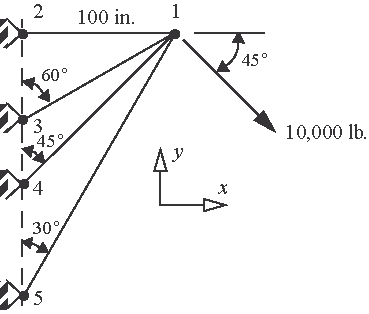
\includegraphics{Figure_6-23.pdf}
}
{\caption{Four bar truss of exercise 1.\label{fig6.23}}}
}

\processfigure{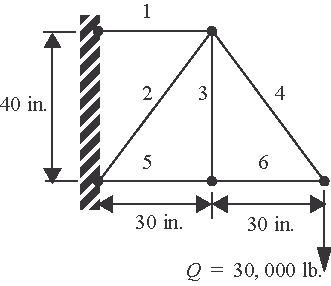
\includegraphics{Figure_6-24.pdf}
}
{\caption{Six-bar truss for exercises 2 and 3.\label{fig6.24}}}

\item[\textbf{3.}] Use Castigliano's’ second theorem to compute the horizontal displacement of the right-hand joint of exercise~2.

\item[\textbf{4.}] The truss shown figure~\ref{fig6.25} consists of three bars: 1-4, 2-4, and 3-4. Each bar has the same cross-sectional area $A$, modulus of elasticity $E$, and the same coefficient of thermal expansion $\alpha$. Bar 1-4 is subjected to a change in temperature $\Delta$T from ambient temperature (the unstressed state), while bars 2-4 and 3-4 remain at ambient temperature. Use Castigliano's first theorem to determine the horizontal displacement $q_7$ and the vertical displacement $q_8$ of joint 4.

{\def\floatbelowskip{-3pt}%
\processfigure{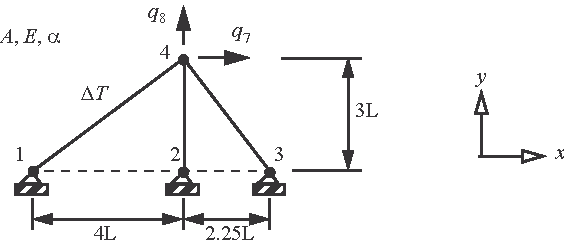
\includegraphics{Figure_6-25.pdf}
}
{\caption{Three-bar truss of exercise~4.\label{fig6.25}}}}

\item[\textbf{5.}] The plane truss shown in figure~\ref{fig6.26} represents a single bay of a wing spar truss. For all bars: $E=75\,\mathrm{GPa}$ and $\alpha=23.0 \times 10^{-6} /{ }^{\circ} \mathrm{C}$. The cross-sectional areas of the bars are: 2580 mm$^2$ for the horizontal bars,\vadjust{\vspace*{10pt}\pagebreak} 387 mm$^2$ for the vertical bars, and 2690 mm$^2$ for the diagonal bars. The upper horizontal bar is heated to $250^{\circ} \mathrm{C}$ above the zero stress temperature, and all other bars remain at the zero stress temperature. Two 45 kN lift forces act at joints 1 and 2.

{\floataboveskip=-1pc
\floatbelowskip=-0.6pc
\processfigure{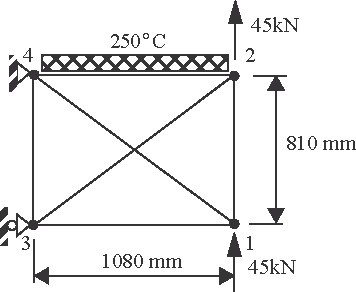
\includegraphics{Figure_6-26.pdf}
}
{\caption{Six-bar truss in a single bay of a wing spar.\label{fig6.26}}}}

\vspace*{-10pt}

Use Castigliano's first theorem to find
\begin{enumerate}[b)]
\item[{\hskip13pt}a)] stiffness matrix in kN/mm,
\item[{\hskip13pt}b)] displacement of all joints in mm,
\item[{\hskip13pt}c)] all boundary reactions in kN, and
\item[{\hskip13pt}d)] the stresses in MPa in each bar.
\end{enumerate}

\item[\textbf{6.}] The truss shown in figure~\ref{fig6.27} consists of five bars: 1-2, 1-3, 1-4, 2-4, and 3-4. Each bar has the same cross-sectional area \textit{A} and same modulus of elasticity \textit{E}. The lengths of bars 1-2, 1-4, and 3-4 are the same, and are denoted by \textit{L}. A horizontal force of magnitude \textit{P} is applied to joint 1. Use Castigliano's second theorem to determine the horizontal displacement $q_5$ of joint 3.

{\floatbelowskip=-0.8pc
\processfigure[!h]{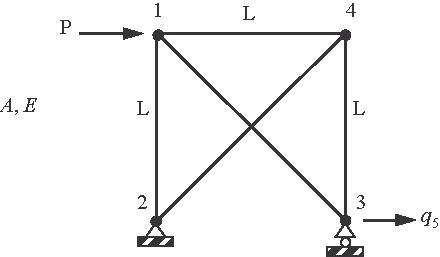
\includegraphics{Figure_6-27.pdf}}
{\caption{Five-bar truss of exercise~6.\label{fig6.27}}}}

\item[\textbf{7.}]  A simply supported, uniform beam of length \textit{L} is subjected to a moment $Q_{1}$ at its left end as shown in figure~\ref{fig6.28}. The material is homogeneous and linear elastic, the cross section is symmetric ($I_{x y}=0$), and there are no thermal strains. The bending stiffness is \textit{EI}. Use Castigliano's second theorem to determine the rotation at \textit{(a)} the left end, and \textit{(b)} the right end. Neglect energy due to transverse shear deformation.

%\clearpage

{\floataboveskip=-0.6pc
\processfigure[!h]{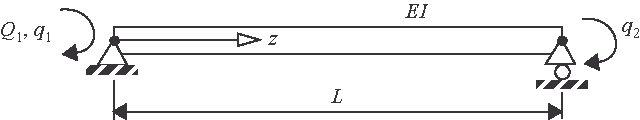
\includegraphics{Figure_6-28.pdf}}
{\caption{Simply supported beam of exercise~7.\label{fig6.28}}}}

\item[\textbf{8.}] A coplanar frame is subjected to an end force $Q_{1}$ as shown in figure~\ref{fig6.29}. The bars of the frame are uniform with axial stiffness \textit{EA} and bending stiffness \textit{EI}. Use Castigliano's second theorem to find
\begin{enumerate}[b)]
\item[{\hskip13pt}a)] the end rotation $q_{2}$, and
\item[{\hskip13pt}b)] the vertical displacement $q_{3}$ at the joint.
\end{enumerate}

{\floataboveskip=-1pc
\floatbelowskip=-0.6pc
\processfigure[!h]{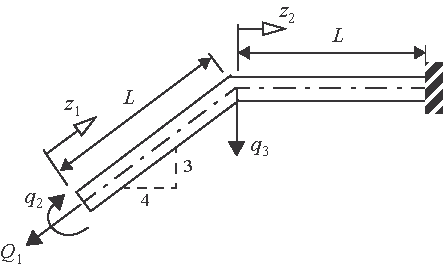
\includegraphics{Figure_6-29.pdf}}
{\caption{Coplanar frame.\label{fig6.29}}}}

\item[\textbf{9.}] Consider the statically indeterminate, uniform beam shown in figure~\ref{fig6.30} that is subjected to a uniform, downward distributed load of intensity $p$. For small displacements assume that only the complementary strain energy in bending is significant. If the center support moves downward by the amount $0.01 p L^{4}/E I_{x x}$ and remains attached to the beam, use Castigliano's second theorem to find the reactions at the left and right supports.

{\floataboveskip=-1pc
\floatbelowskip=-0.6pc
\processfigure[!h]{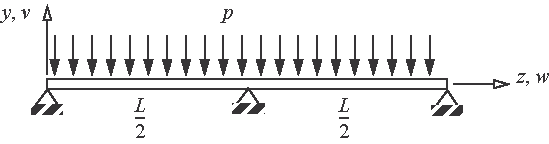
\includegraphics{Figure_6-30.pdf}
}
{\caption{Uniform beam of exercise~9.\label{fig6.30}}}}

\item[\textbf{10.}] The frame consists of three slender, uniform bars of length $L$, and two right angle bends. Assume the bends are rigid joints. Each member has a solid circular cross section of diameter $d$. A force $P$ acts in the global $X$-direction at point A. Find the three displacement components $u_{A}, v_{A}, w_{A}$ of point A in terms of $P$, $L$, $d$, and $E$ using Castigliano's second theorem. Assume $G=0.4 E$. Neglect deformations due to transverse shear.

{\floataboveskip=-1pc
\floatbelowskip=-0.6pc
\processfigure[!h]{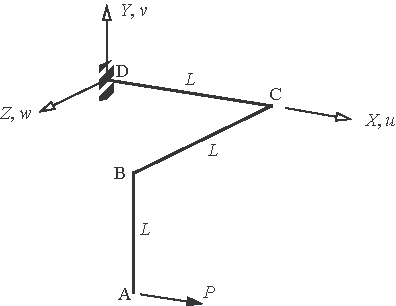
\includegraphics{Figure_6-31.pdf}
}
{\caption{Space frame of exercise~10.\label{fig6.31}}}}

\pagebreak

\item[\textbf{11.}] The rectangular space truss shown in the sketch consists of six bars: 1-2, 1-3, 1-4, 2-3, 2-4, and 3-4. The cross-sectional area of each bar is 200 mm$^2$. The temperature of bar 2-3 is increased by $30^{\circ} \mathrm{C}$ above the stress free temperature, while the other five bars remain at the stress free temperature. Calculate the forces in all six bars. The coefficient of thermal expansion $\alpha=7 \times 10^{-6} /{ }^{\circ} \mathrm{C}$, and the modulus of elasticity $E=200 \times 10^{3}\,\mathrm{N} / \mathrm{mm}^{2}$.


\processfigure[!h]{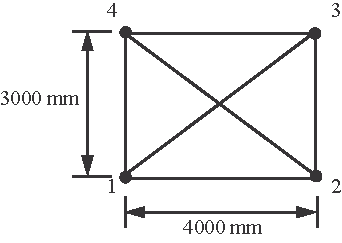
\includegraphics{Figure_6-32.pdf}
}
{\caption{Space truss of exercise~11.\label{fig6.32}}}


\noindent Note that $m=6$, $j=4$, and $r=0$. Hence, $m<2 j-r$, and this truss cannot support an external load without accelerating. However, under the self-straining caused by the temperature change, it is statically indeterminate internally.


\item[\textbf{12.}]  Sketch the bending moment diagrams of bars 1-2 and 2-3 in the singly redundant frame shown in figure~\ref{fig6.33}. Each bar has the same length \textit{L} and flexural stiffness \textit{EI}. Since the bars are slender, neglect deformations due to extension and transverse shear. Take the reaction moment at support point 1 as the redundant.

{\def\floatbelowskip{-3pt}%
\processfigure[!h]{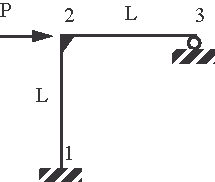
\includegraphics{Figure_6-33.pdf}
}
{\caption{Two-bar frame of exercise~12.\label{fig6.33}}}}

\item[\textbf{13.}]  The aerodynamic advantages of high aspect-ratio (AR) wings are well known---long span reduces lift-induced drag and narrow chord promotes laminar flow to reduce skin-friction drag. However, a long wing span significantly increases the structural loads at the wing root requiring heaver components to safely transmit the loading to the fuselage. The truss-braced wing (TWB) is a method to reduce the load at the wing root. (It is the subject of research in AOE at Virginia Tech under a NASA program to achieve significant fuel savings for 737 type airplanes (Warwick, 2011)). A simplified model of TWB in this exercise is a single truss bar supporting a wing spar.

\bigskip

A wing spar is clamped at its root and supported by a truss bar that is pinned to the support at one end and pinned to the spar at the other end. Refer to figure~\ref{fig6.34}. The spar is subjected to a span-wise distributed air load $f_{y}(z)$ approximated by
\setcounter{equation}{0}\def\theequation{\alph{equation}}
\begin{align}
f_{y}(z)=\frac{3 L}{2 b}\left[1-\left(\frac{z}{b}\right)^{2}\right] \quad 0 \leq\left(\frac{z}{b}\right) \leq 1.
\end{align}
where the lift on the wing is denoted by \textit{L} and the wing span is denoted by $b$. The pin connection of the truss bar to the spar is at the span-wise distance $s \cdot b$ from the root, where the range of nondimensional parameter $s$ is $0<s \leq 1$.

\medskip

The assemblage is statically indeterminate, and the statically determinate base structure is obtained by removing the lower pin support of the truss bar and replacing it by the redundant force $Q$ which is also the tensile force in the truss bar. Refer to the right-hand sketch in figure~\ref{fig6.34}. The condition of compatibility is the displacement corresponding to the redundant is equal to zero. Enforce compatibility by Castigliano's second theorem given by
\begin{align}
q=\frac{\partial U^{*}}{\partial Q}=0 \quad U^{*}=\int_{0}^{s b}\left(\frac{M_{x}^{2}}{2 E I_{x x}}+\frac{N^{2}}{2 E A}\right) d z+\int_{s b}^{b}\left(\frac{M_{x}^{2}}{2 E I_{x x}}\right) d z+\frac{Q^{2} l_{s}}{2 E A_{s}}.
\end{align}
where $l_{s}$ is the length of the strut. Numerical data are listed in table~\ref{tab6.7}.

\processfigure[!h]{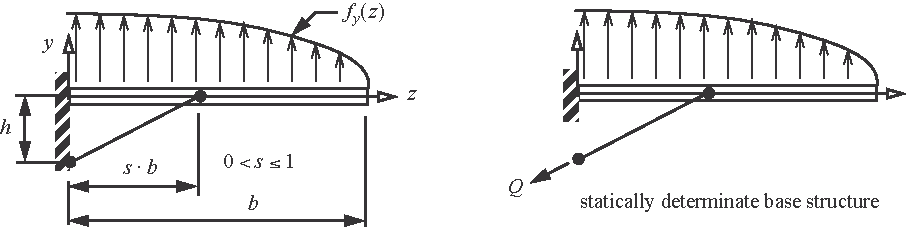
\includegraphics{Figure_6-34.pdf}
}
{\caption{Truss-braced wing.\label{fig6.34}}}

\begin{enumerate}[b)]
\item[{\hskip13pt}a)] Plot the normalized bending moment at the wing root $\left(M_{x}(0)\right) / M_{0}$ versus $s$ for $0.01 \leq s \leq 1$, where $M_{0}$ is the root bending moment of the cantilever wing; i.e., $M_{0}=-(3 / 8) b L$

\item[{\hskip13pt}b)] Plot the tensile normal stress $\sigma=Q / A_{s}$ in the strut versus $s$ for $0.01 \leq s \leq 1$.

\item[{\hskip13pt}c)] If the allowable tensile stress in the strut is 30 ksi, what is the value of $s$ to yield the smallest value of the ratio $\left(M_{x}(0)\right) / M_{0}$? What is the value of $\left(M_{x}(0)\right) / M_{0}$ for this particular $s$?
\end{enumerate}

\begin{table}[!h]
\processtable{Numerical data for the strut-braced wing\label{tab6.7}}
{\begin{tabular}{@{}ll@{}}
\toprule
$b$, wing span & 390 in. \\
$h$, vertical distance from the spar centroid to lower strut support &72 in. \\
\textit{A}, cross-sectional area of the spar &23.88 in.$^2$ \\
$I_{xx}$, second area moment of the cross section of the spar &872.716 in.$^4$ \\
$A_s$, cross-sectional area of the strut (1.75 in. diameter) &2.40528 in.$^2$ \\
$L$, wing lift &50,000. lb. \\
$E$, modulus of elasticity for the spar and strut material &$10 \times 10^{6} \text { 1b./in.}{}^{2}$ \\
\botrule
\end{tabular}}{}
\end{table}

\end{enumerate}
\end{exercise}

\end{document}